% LaTeX-Vorlage Medizintechnik Projektarbeit
% Alexander Ruppel
% veraendert von Eva Eibenberger 
% veraendert von Stephan Seitz

% %%%%%%%%%%%%%%%%%%%%%%%%%%%%%%%%%%%%%%%%%%%%%%%%%%%%%%
% Please change the title of the project work, add your name 
% and matriculation number and set the language of your project 
% report 
% %%%%%%%%%%%%%%%%%%%%%%%%%%%%%%%%%%%%%%%%%%%%%%%%%%%%%%
\documentclass[%
	a4paper, %
	12pt, %
	english, % set to english if you want to write in English
	bibtotoc %
]{scrartcl}

% Gruppe: Nummer der Projektarbeit

% Thema der Projektarbeit
\newcommand{\titel}{Fundamental Image Processing Techniques in Biomedical Imaging}

% Studentenname und Matrikelnummer 
\newcommand{\erster}{Muhammad Muaviya Ijaz}		% Student 1: Vorname Nachname
\newcommand{\mnreins}{23454875}		% Student 1: Matrikelnummer

\newcommand{\todo}[1]{{\color{blue}{TODO: {#1}}}} 
\newcommand{\sltn}[1]{{\color{red}{SOL: {#1}}}} 
\usepackage{xcolor}
\usepackage{enumitem}
\usepackage{float}
\usepackage{subcaption} % For subfigures
\usepackage{graphicx}


% in header Spache einstellen!
% LaTeX-Vorlage Medizintechnik Projektarbeit
% Wintersemster 2009/10
% Alexander Ruppel
% veraendert von Eva Eibenberger 

%% Seitenraender
\usepackage[head=12.5mm,headsep=12mm,left=25mm,right=25mm,top=28mm,bottom=20mm]{geometry} 

%% Absatzeinstellungen
\setlength{\parindent}{0em} % Einrueckung neuer Absaetze

%% Kopf- und Fusszeilen
\usepackage{scrlayer-scrpage}
\pagestyle{scrheadings}
\clearscrheadings{} %
\clearscrplain{}	  %
\clearscrheadfoot{} % Kopf- und Fuzeilen werden geloescht
\renewcommand{\headfont}{\normalfont\small}
\ihead{\titel{}}
\ohead{\pagemark}

%% Zeichenkodierung
\usepackage[utf8]{inputenc}
\usepackage{babel,fixltx2e}
\usepackage[T1]{fontenc}

\usepackage[babel]{csquotes}
%% Literaturverzeichnis
%\usepackage[square,authoryear]{natbib}
%\renewcommand{\cite}{\citep}

%% Schriftart
\usepackage{helvet}
\renewcommand{\familydefault}{\sfdefault} % Standardschrift auf sf setzen
\usepackage{textcomp}

%% Tabellen
\usepackage{tabularx}
\usepackage{multirow,multicol}

%% Captions
\usepackage[margin=2em,format=plain,indention=.8em,labelsep=quad,font=small,labelfont=bf,textfont=it]{caption}
\usepackage{breakcites}

%% Mathe & Co
\usepackage{amsmath,amssymb,amsfonts}

%% Grafiken
\usepackage{graphicx}
\graphicspath{{Grafiken/}}
\usepackage{wrapfig}

%% PDF-Optionen
\usepackage[
    bookmarks,
    bookmarksopen=true,
    colorlinks=true,
% diese Farbdefinitionen zeichnen Links im PDF farblich aus
    %linkcolor=red, % einfache interne Verknpfungen
    %anchorcolor=black,% Ankertext
    %citecolor=blue, % Verweise auf Literaturverzeichniseintrge im Text
    %filecolor=magenta, % Verknpfungen, die lokale Dateien ffnen
    %menucolor=red, % Acrobat-Menpunkte
    %urlcolor=cyan, 
% diese Farbdefinitionen sollten fr den Druck verwendet werden (alles schwarz)
    linkcolor=black, % einfache interne Verknpfungen
    anchorcolor=black, % Ankertext
    citecolor=black, % Verweise auf Literaturverzeichniseintrge im Text
    filecolor=black, % Verknpfungen, die lokale Dateien ffnen
    menucolor=black, % Acrobat-Menpunkte
    urlcolor=black, 
    backref, % zurückverweise im Inhaltsverzeichnis auf die Seite
    plainpages=false, % zur korrekten Erstellung der Bookmarks
    pdfpagelabels, % zur korrekten Erstellung der Bookmarks
    hypertexnames=false, % zur korrekten Erstellung der Bookmarks
    linktocpage % Seitenzahlen anstatt Text im Inhaltsverzeichnis verlinken
]{hyperref}

%% Diverses
\usepackage{nameref}
\usepackage{blindtext}
\usepackage{ifthen}

\setlength{\parskip}{\baselineskip}%
\setlength{\parindent}{0pt}%


\begin{document}

% LaTeX-Vorlage Medizintechnik Projektarbeit
% Wintersemster 2009/10
% Alexander Ruppel
% veraendert von Eva Eibenberger 
% veraendert von Paul Stöwer
% veraendert von Mischa Dombrowski

% %%%%%%%%%%%%%%%%%%%%%%%%%%%%%%%%%%%%%%%%%%%%%%%%%%%%%%
% Diese Datei muss NICHT veraendert werden
% %%%%%%%%%%%%%%%%%%%%%%%%%%%%%%%%%%%%%%%%%%%%%%%%%%%%%%

\begin{titlepage}

\begin{center}
Friedrich-Alexander-Universit\"at Erlangen-N\"urnberg\\
Artificial Intelligence in Biomedical Engineering\\
W3-Professur für Image Data Exploration and Analysis\\
Prof.\ B.\ Kainz\\
W3-Professur für Computational Imaging\\
Prof.\ F.\ Knoll\\


\vspace*{9em}

{\huge \textbf{\textsf{Medizintechnik II}}}\\[.3em]
{Projektarbeit}\\[.3em]
{Sommersemester 2024}\\

\vspace*{9em}

{\huge \textbf{\textsf{\titel}}}\\[.7em]
{\today}
\end{center}

\vfill% {
\begin{tabbing}
	\hspace*{5cm} \= Vorname Nachname \hspace*{4em} \= Matrikelnummer \kill
	Studierende*r:\> \erster \> \mnreins \\
%	\ifthenelse{\equal{\student}{\erster}}{\textbf{\erster} \> \textbf{\mnreins}}{\erster \> \mnreins} \\
%	\ifthenelse{\equal{\student}{\zweiter}}{\textbf{\zweiter} \> \textbf{\mnrzwei}}{\zweiter \> \mnrzwei} \\
%	\ifthenelse{\equal{\student}{\dritter}}{\textbf{\dritter} \> \textbf{\mnrdrei}}{\dritter \> \mnrdrei} \\
%	\ifthenelse{\equal{\student}{\vierter}}{\textbf{\vierter} \> \textbf{\mnrvier}}{\vierter \> \mnrvier} \\
%	\ifthenelse{\equal{\student}{\fuenfter}}{\textbf{\fuenfter} \> \textbf{\mnrfuenf}}{\fuenfter \> \mnrfuenf} \\
\end{tabbing}
%}

\end{titlepage}


% Inhaltsverzeichnis
\tableofcontents
\newpage

% Dateien, die den Text enthalten
\section{Introduction}%
\label{sec:introduction}

\begin{figure}
    \centering
    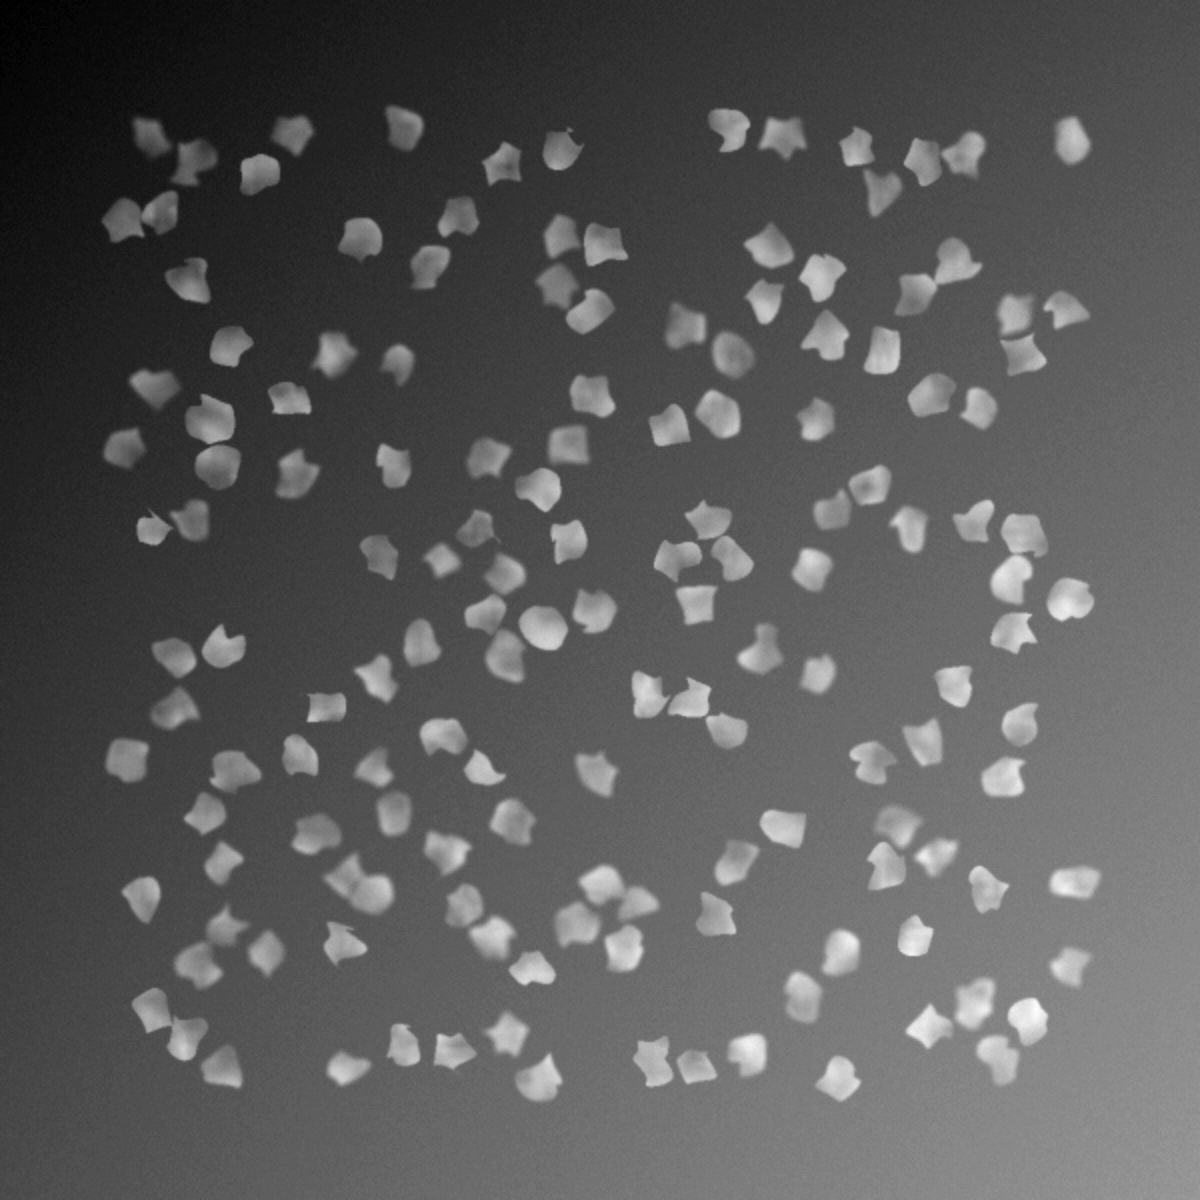
\includegraphics[width=0.3\linewidth]{cells.png}
    \caption{Grayscale Image showing clusters of cells}
    \label{fig:figurecell}
\end{figure}


In the progressing field of biomedical engineering, \textbf{Image Processing} plays a vital role in enhancing medical diagnostics and research. Basic methods such as thresholding, segmentation, and edge detection are crucial for improving and examining biomedical images, like those showing cellular structures. These fundamental techniques are essential instruments for biomedical engineers, allowing them to enhance image quality and obtain valuable data, consequently influencing the precision of diagnoses and research results.

This report goal is to present \textbf{key image processing techniques} that can be applied directly to cellular imaging, offering practical knowledge. This study underscores the importance of these methods in analyzing biomedical images by linking theoretical concepts to practical applications. The primary emphasis is on basic methods such as thresholding, Otsu's algorithm, segmentation and its evaluation, and edge detection, serving as the foundation for advanced image analysis tools like Fourier Transform filtering, Transfer learning, and Convolutional Neural Networks (CNNs). Having a strong grasp of these fundamental skills is essential for advancing to more complex techniques and creating innovative algorithms in the field of biomedical imaging.

The efficient processing and analysis of biomedical images to extract meaningful and correct information is the \textbf{primary goal} of this report. In particular, the report concentrates on describing and evaluating various image segmentation algorithms for the purpose of analyzing and identifying cellular features as portrayed by the provided cells image, shown in Figure \ref{fig:figurecell}. The \textbf{main research question} is: "How can basic image processing techniques be applied to biomedical images, such as those depicting cellular structures, to enhance the efficiency and accuracy of segmentation?" This, in turn, will enhance the overall analysis and interpretation of biomedical data. \textbf{ChatGPT} is used as a writing assistant in this report to enhance paragraph-level grammar, spellchecking of the content, and improve the clarity of explanations. However, the content, analysis, and conclusions presented are entirely by our own research \cite{openai_gpt4}.

Figure \ref{fig:figurecell} shows an image of cluster of cells. In the following parts, we will explore the precise techniques as mentioned before in the report. The evaluation of these methods' efficacy will be based on how they are used with this original image of cells.

\section{Method}
\subsection{Thresholding and Illumination-Correction}
\label{sec: thresholding_and_illumination_correction}

In this section, we explain the basic techniques like \textbf{Basic Thresholding} and \textbf{Illumination Correction} in microscopy images. These techniques are crucial for enhancing image analysis by transforming grayscale images into binary images and fixing the problem of uneven illumination, a frequent occurrence in microscopy. The procedure includes transforming an 8-bit grayscale picture into a binary image using a threshold value set by the user. Moreover, a supplementary measure is taken to address the problem of uneven illumination, a frequent issue encountered in microscopy imaging. To demonstrate these techniques,we take the example of the image of cells again, as shown in Figure \ref{fig:figurecell}.

\textbf{Thresholding} is a basic method in image processing which changes a grayscale image to a binary image. Thresholding aims to divide the image into black and white regions by assessing pixel intensity values, distinguishing between foreground and background. This technique is particularly beneficial in binarization of the image, facilitating further image analysis like segmentation or object detection \cite{gonzalez_digital_image_processing}.

Basic thresholding involves the user selecting a specific intensity threshold, $t$, during the process. The intensity value, $I(x, y)$, of each pixel in the grayscale image is checked against the threshold $t$. After comparing, the pixel is categorized as foreground or background. The outcome is an image that is binary. The \textbf{mathematical representation of using thresholding} for image binarization, as mentioned and discussed in the survey \cite{sahoo_survey_thresholding_techniques}, can be expressed as:

\begin{equation}
T(x, y) = 
\begin{cases} 
b_1 & \text{if } I(x, y) > \text{t} \\
b_0 & \text{otherwise}
\end{cases}
\label{eq:thresholding}
\end{equation}

where x and y and the the coordinates in the Image I for a specific pixel value and variables \(b_1\), \(b_0\)  represents values for white and black color respectively. If the pixel value is greater than the 
threshold value t, that pixel location is set value of 255 i.e white, otherwise 0 i.e black.

Another issue which happens to be there in microscopy images is of \textbf{Uneven Illumination}. It can result in incorrect analysis because of gradients or vignetting effects. In order to fix this issue, we adjust the image's brightness by dividing it by a blurred version that signifies the lighting variation. Mathematically speaking, this is represented in the form of the following equation:

\begin{equation}
C(x, y) = \frac{I(x, y)}{B(x, y)}
\label{eq:illuminationcorrection}
\end{equation}

where \( C(x, y) \) is the corrected pixel value, \( I(x, y) \) is the original pixel value, and \( B(x, y) \) is the blurred image. The blur, achieved with a large-radius Gaussian filter, captures the illumination gradient, effectively correcting the image. The advanced form of this method is also cited in this article \cite{smith_illumination_correction_method} where they employed a model-based approach that handled complex and varying illumination variations across approximate 11 datasets. 

Ensuring accurate analysis in microscopy is essential through illumination correction to prevent gradients and vignetting that can obscure details. Vignetting decreases brightness or saturation around the edges of an image, usually caused by problems with the light transmission from the microscope to the camera. Distortions of this kind can result in inaccuracies in quantitative measurements and impact tasks such as image segmentation and mosaicking. It is crucial to rectify these artifacts to prevent inaccurate outcomes in medical diagnosis. Recent techniques, such as a Fully Convolutional Network (FCN) with feature encoding, decoding, and detail supplementation, have shown to be successful. This method, when applied to pathological cell images, surpasses conventional techniques, enhancing image mosaicking and visual quality \cite{wang_fcn_microscopic_image_illumination_correction}.

The following figures showcase example of microscopy image  before and after thresholding done on Figure \ref{fig:figurecell}, with and without illumination correction, based on calculations of above mentioned Equations \ref{eq:thresholding} and \ref{eq:illuminationcorrection}, implemented in our project.

\begin{figure}[H]
    \centering
    \begin{subfigure}[b]{0.3\textwidth}
        \centering
        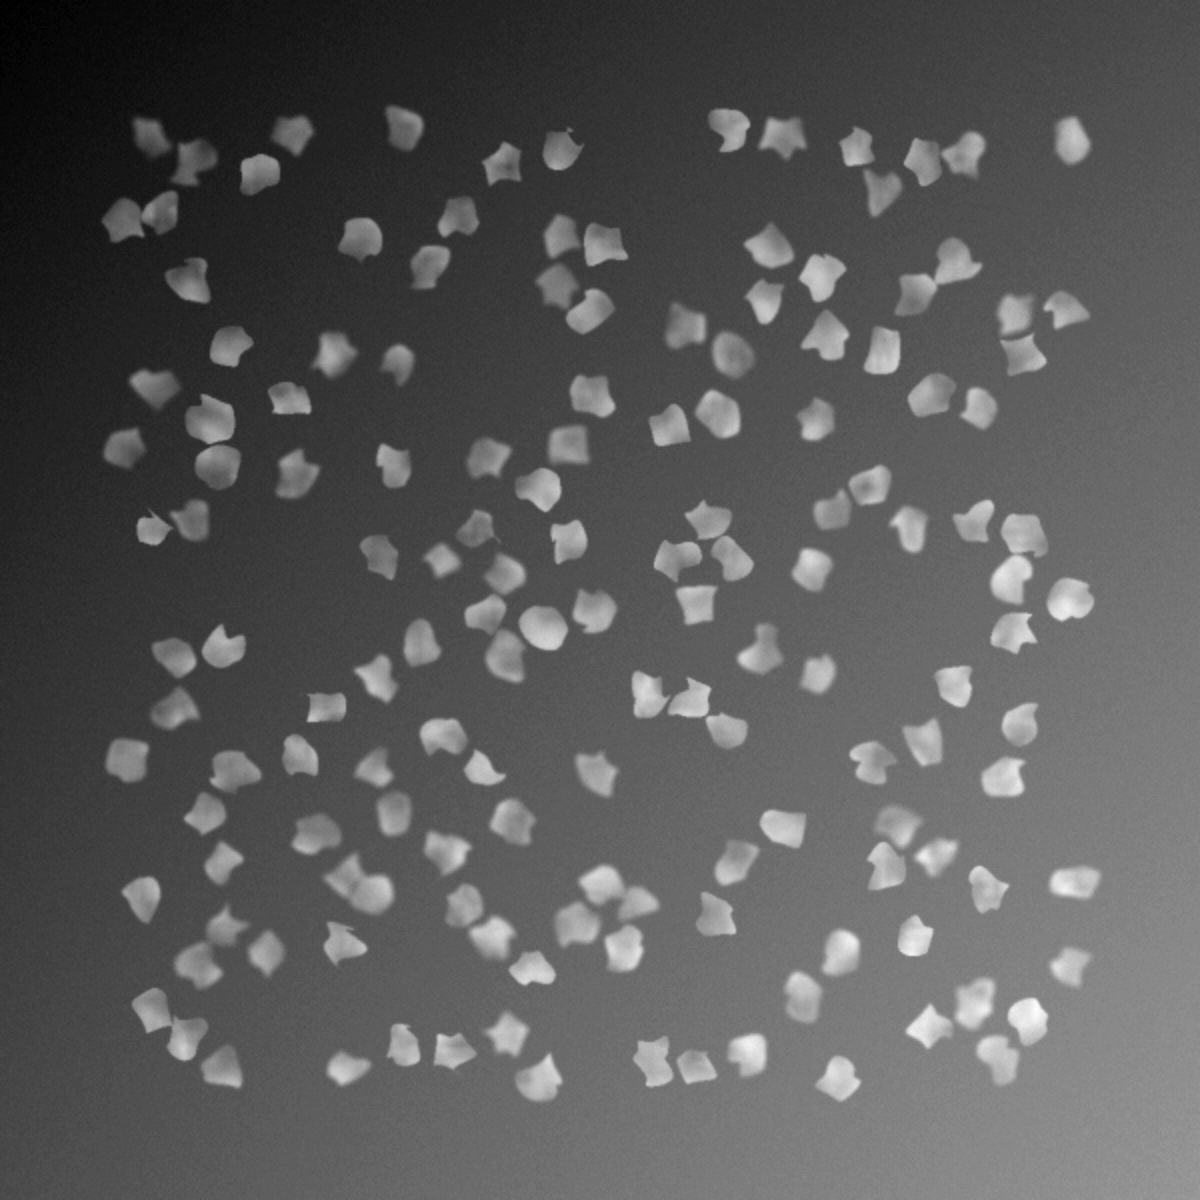
\includegraphics[width=\textwidth]{cells.png}
        \caption{Original Image}
        \label{fig:original_img}
    \end{subfigure}
    \hspace{1cm} % Adjust space between images as needed
    \begin{subfigure}[b]{0.3\textwidth}
        \centering
        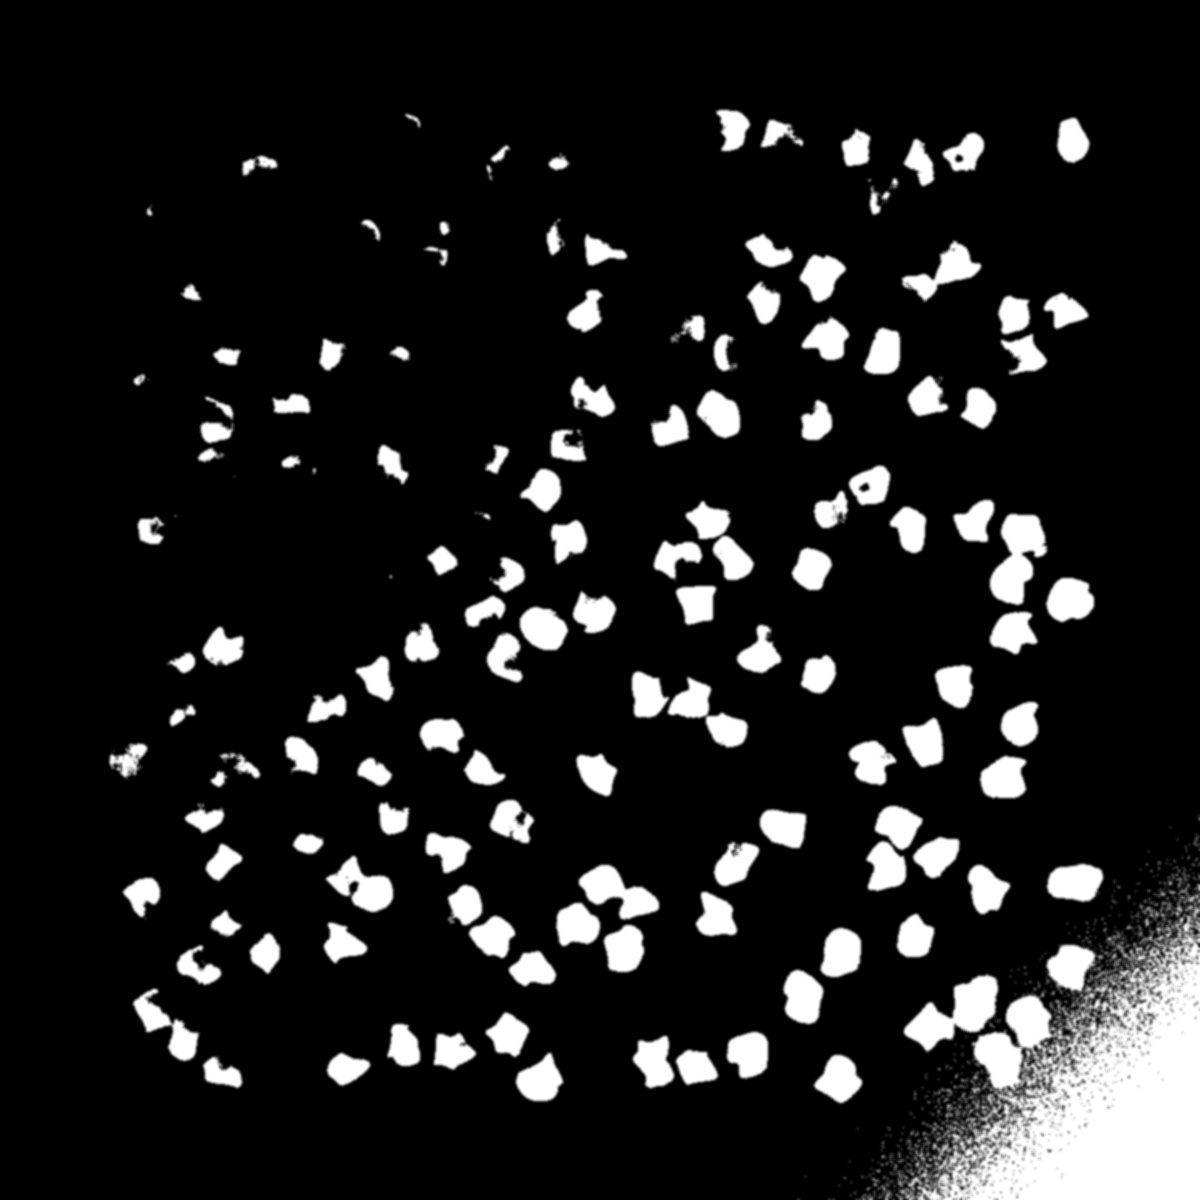
\includegraphics[width=\textwidth]{cells_thresholding.jpg}
        \caption{Image After Thresholding}
\label{fig:thresholded_img_without_illumination}
    \end{subfigure}
    \caption{Comparison of images before and after thresholding with t = 135}
    \label{fig:comparison_before_illumination}
\end{figure}

Figure \ref{fig:comparison_before_illumination} compares the original microscopy image, shown in Figure \ref{fig:original_img} with its thresholded version, shown in Figure \ref{fig:thresholded_img_without_illumination}  using a threshold value of \( t = 135 \). The thresholding was applied without prior illumination correction, resulting in inaccuracies, particularly near the image edges due to uneven lighting in the original image.

\begin{figure}[H]
    \centering
    \begin{subfigure}[b]{0.3\textwidth}
        \centering
        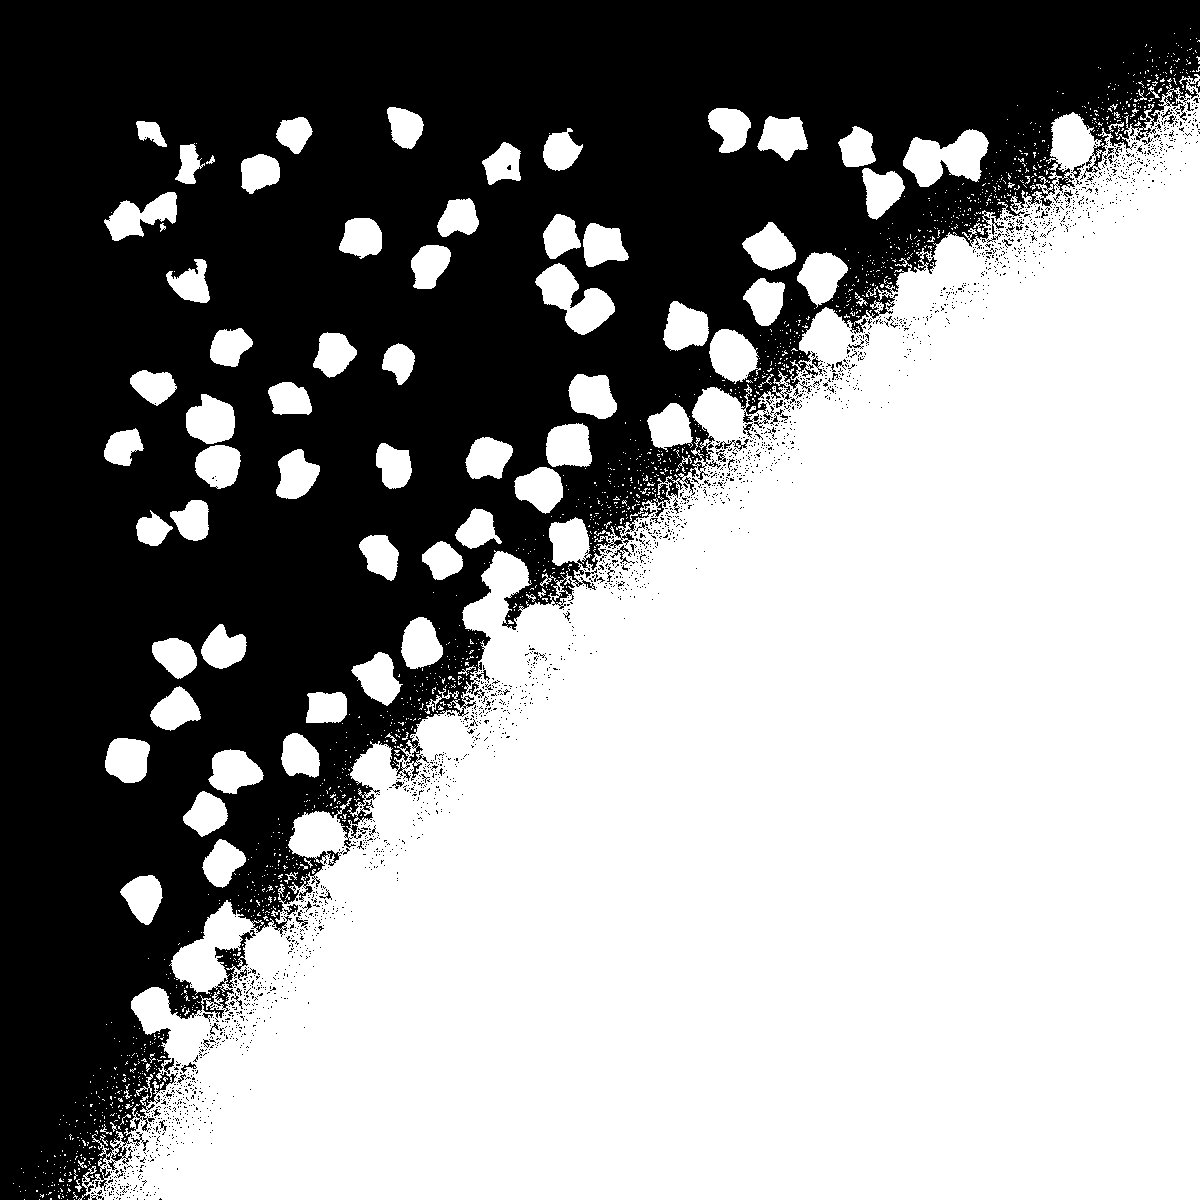
\includegraphics[width=\textwidth]{uneven_illuminated img.jpg}
        \caption{Uneven Illuminated Image}
        \label{fig:uneven_illuminated_img}
    \end{subfigure}
    \hspace{1cm} % Adjust space between images as needed
    \begin{subfigure}[b]{0.3\textwidth}
        \centering
        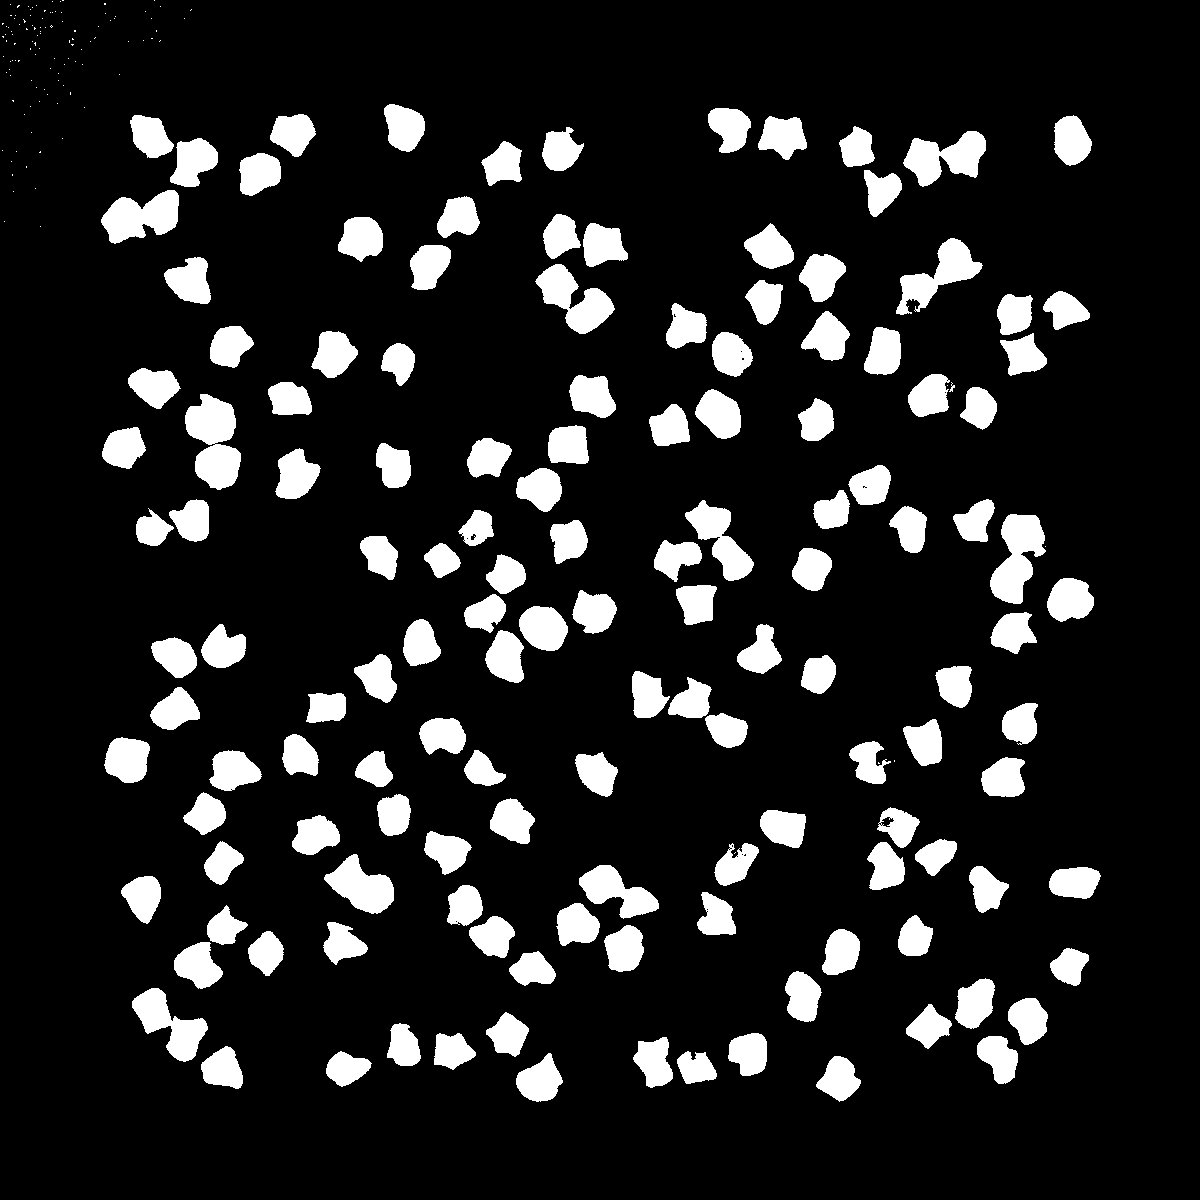
\includegraphics[width=\textwidth]{Illuminated_Thresholded Image.jpg}
        \caption{Illumination Correction}
        \label{fig:illuminated_correction_img}
    \end{subfigure}
    \caption{Comparison of images before and after illumination correction with t = 80}
    \label{fig:comparison_after_illumination}
\end{figure}

Figure \ref{fig:comparison_after_illumination} demonstrates the effect of the \textbf{correctIllumination} method. The original image suffered from uneven illumination as shown in Figure \ref{fig:uneven_illuminated_img}, which caused inaccurate thresholding. After applying the illumination correction, the image intensity was normalized, so that the lighting is evenly distributed across the image, resulting in a more accurate thresholding output, shown in Figure \ref{fig:illuminated_correction_img}.

\subsection{Image Segmentation}
\label{sec:image_segmentation}
In this section, some \textbf{key evaluation metrics} for assessing the results of Image Segmentation in Section \ref{sec: thresholding_and_illumination_correction} will be discussed. We will discuss the metrics such as  True Positives (TP), True Negatives (TN), False Negatives (FN), and False Positives. True Positives (TP) refer to the number of correctly identified pixels that belong to the object. The number of correctly identified pixels as background is shown by True Negatives (TN). If background pixels are incorrectly classified as part of the object, it leads to False Positives (FP), while if object pixels are mistakenly identified as part of the background, it results in False Negatives (FN).

Two key measures for evaluating a segmentation algorithm's effectiveness are Specificity and Sensitivity. These metrics are also used for interpreting diagnostic tests for physician's daily practice \cite{van_diagnostic_methods}. Below are the given formulas:

\begin{equation}
    Specificity = \frac{TN}{TN + FP}  \\
    \label{eq:specificty_formula}
\end{equation}
\begin{equation} 
    Sensitivity = \frac{TP}{TP + FN} \\
    \label{eq:sensitivity_formula}
\end{equation}

When evaluating Image Segmentation, \textbf{Specificity} refers to the percentage of background pixels in the image that are accurately identified. The objective is to achieve a high level of specificity by reducing the number of false positives, making sure that background pixels are not classified as part of the foreground object, as mathematically calculated in Equation \ref{eq:specificty_formula}. Contrary to this, \textbf{Sensitivity} refers to the ratio of correctly identified foreground pixels. A high-quality image segmentation algorithm decreases the number of false negatives by correctly identifying foreground pixels and not misclassifying them as background pixels, as mathematically derived in Equation \ref{eq:sensitivity_formula}. To summarize, these measurements offer a thorough grasp of how well the algorithm works, considering the importance of accurate object detection while also ensuring background is properly excluded. Elevated values for both of these measurements suggest a strong and dependable segmentation procedure.

To evaluate these metrics, we will use the image of cells as shown in Figure \ref{fig:figurecell}
, and then create six different segmentation by applying illumination correction and using various threshold values. Each segmentation will be compared against a reference image, with a focus on evaluating Sensitivity and Specificity. The referenced image which we will use for this task is shown below:

\begin{figure}[H]
    \centering
    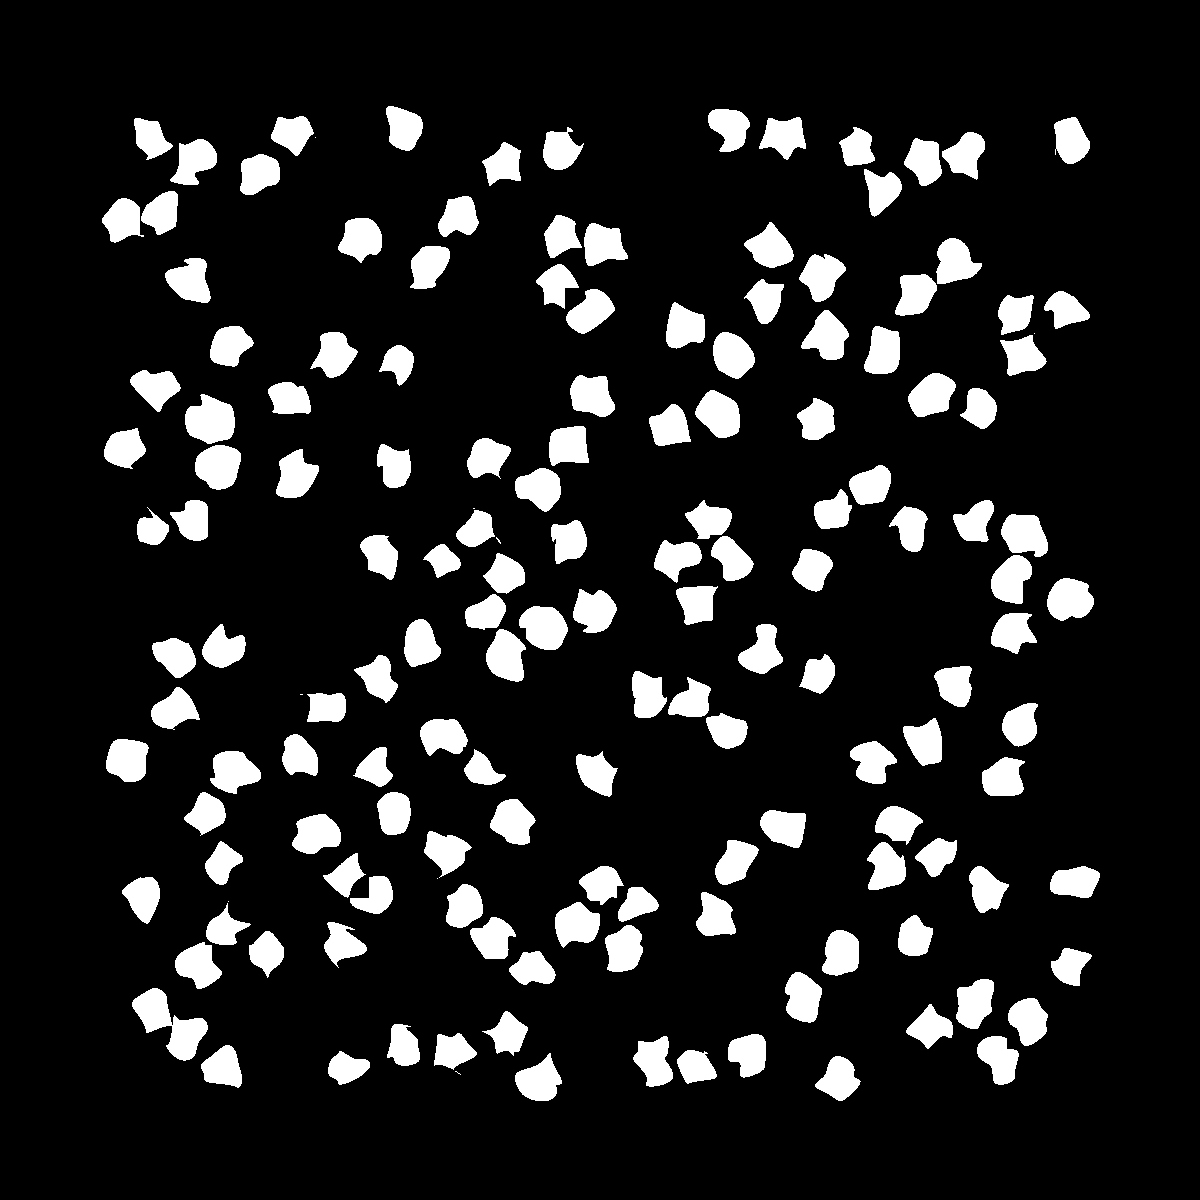
\includegraphics[width=0.3\linewidth]{cells_reference.png}
    \caption{Referenced Cells Image}
    \label{fig:cells_referenced}
\end{figure}

Figure \ref{fig:cells_referenced} shows the image of referenced cells against which we will compare our segmentation results. After performing segmentation on Figure \ref{fig:figurecell}, we got the following results:

\begin{figure}[H]
    \centering
    \begin{subfigure}[b]{0.2\textwidth}
        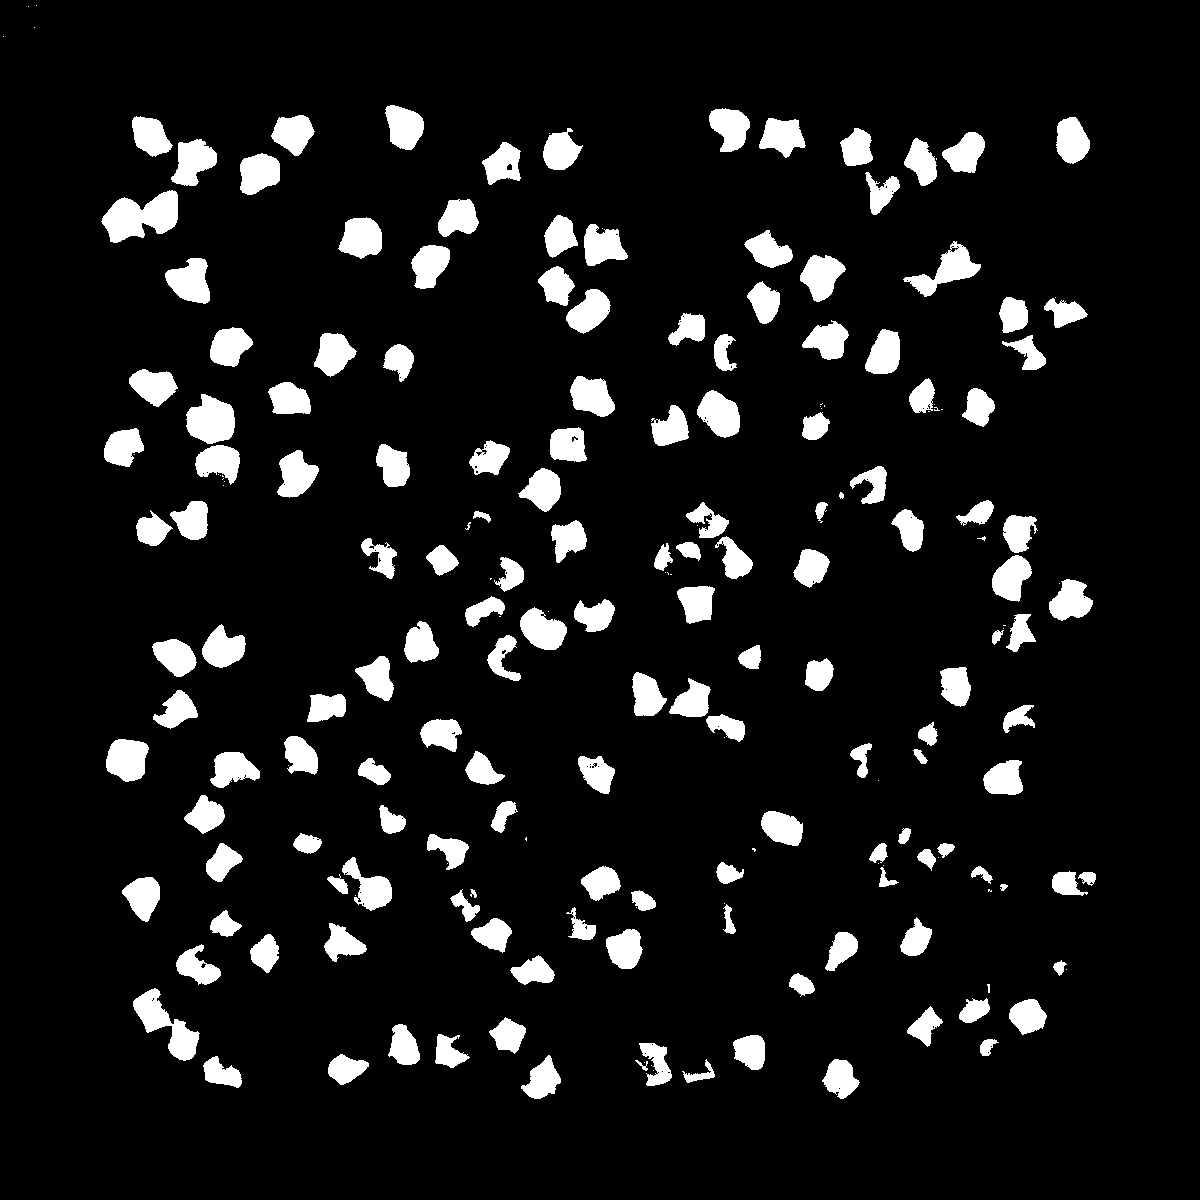
\includegraphics[width=\textwidth]{segmentation_thresholding_92_illuminated.png}
        \caption{Segmentation 1}
        \label{Segmentation1}
    \end{subfigure}
    \hfill
    \begin{subfigure}[b]{0.2\textwidth}
        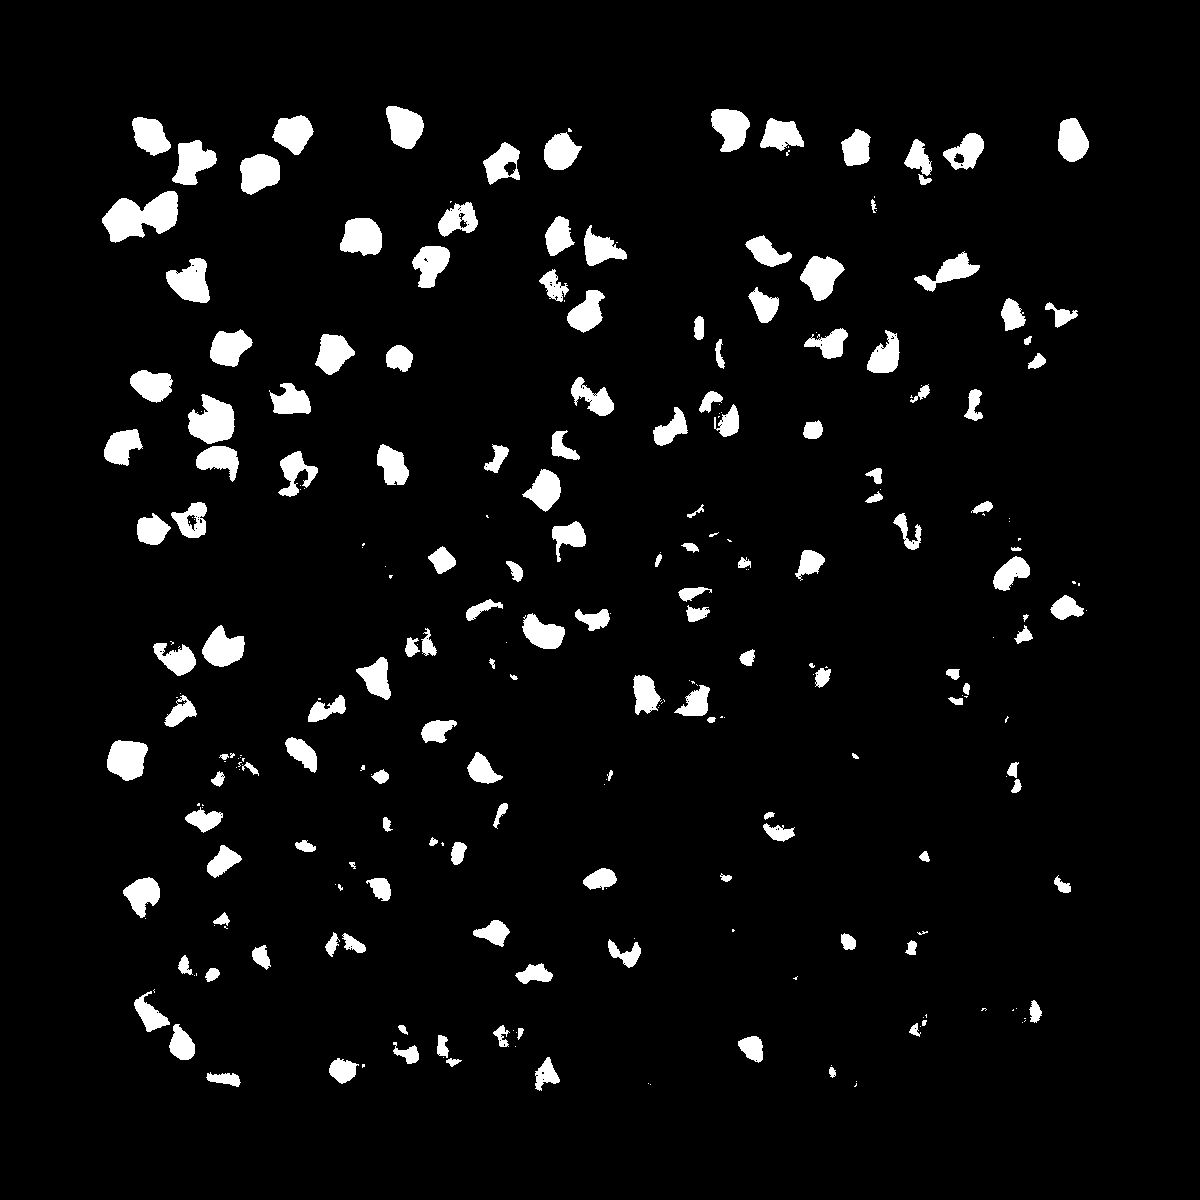
\includegraphics[width=\textwidth]{segmentation_thresholding_105_illuminated.png}
        \caption{Segmentation 2}
        \label{Segmentation2}
    \end{subfigure}
    \hfill
    \begin{subfigure}[b]{0.2\textwidth}
        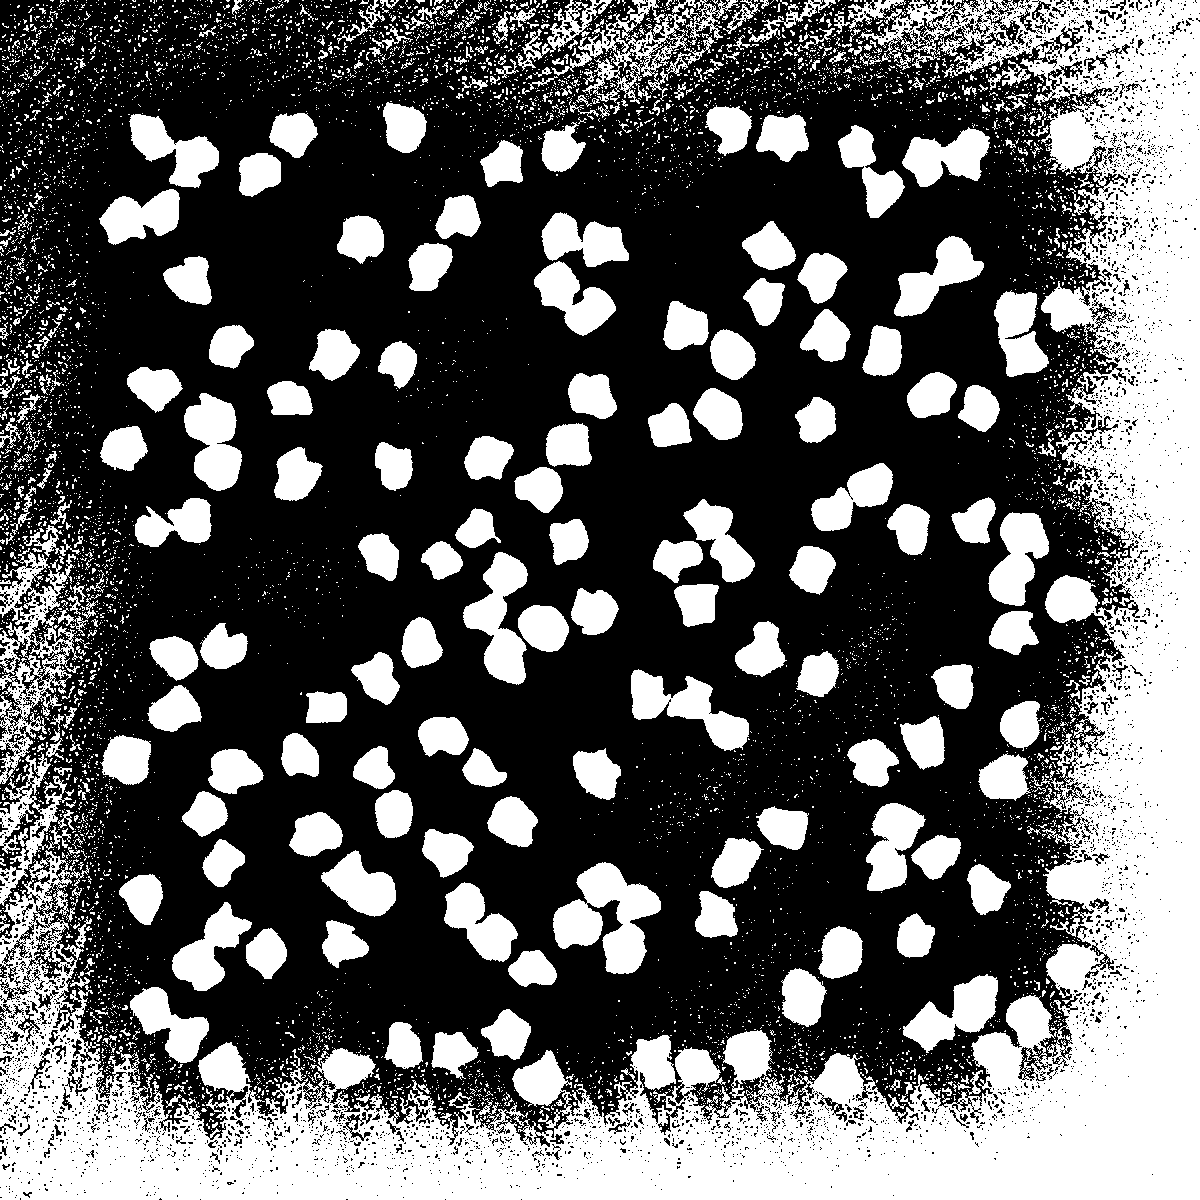
\includegraphics[width=\textwidth]{segmentation_thresholding_60_illuminated.png}
        \caption{Segmentation 3}
        \label{Segmentation3}
    \end{subfigure}

    \vspace{0.5cm}

    \begin{subfigure}[b]{0.2\textwidth}
        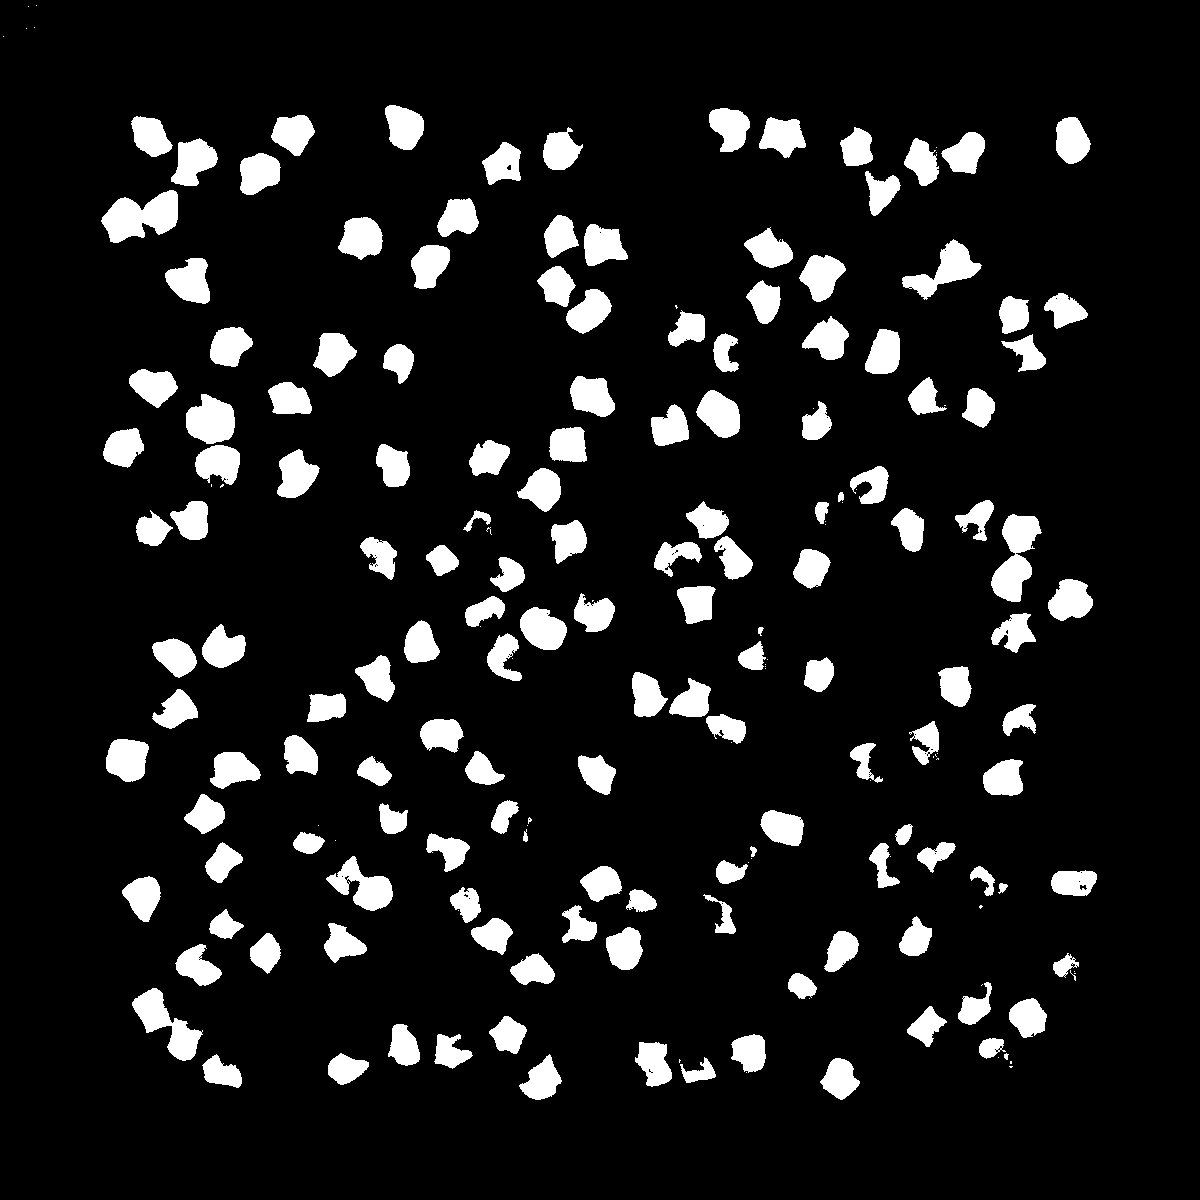
\includegraphics[width=\textwidth]{segmentation_thresholding_88_illuminated.png}
        \caption{Segmentation 4}
        \label{Segmentation4}
    \end{subfigure}
    \hfill
    \begin{subfigure}[b]{0.2\textwidth}
        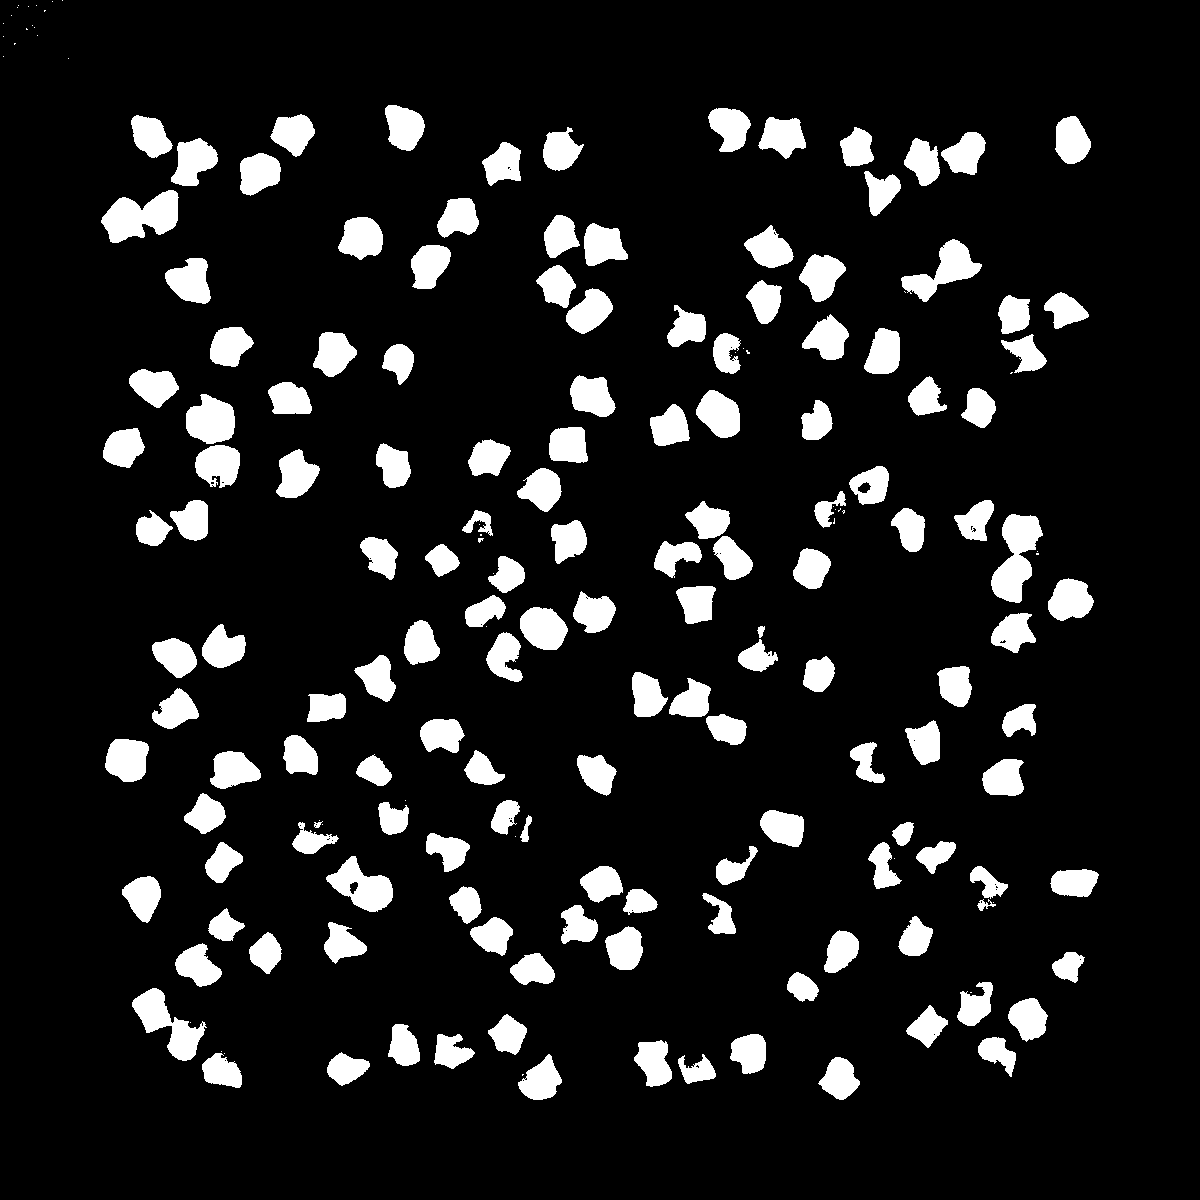
\includegraphics[width=\textwidth]{segmentation_thresholding_84_illuminated.png}
        \caption{Segmentation 5}
        \label{Segmentation5}
    \end{subfigure}
    \hfill
    \begin{subfigure}[b]{0.2\textwidth}
        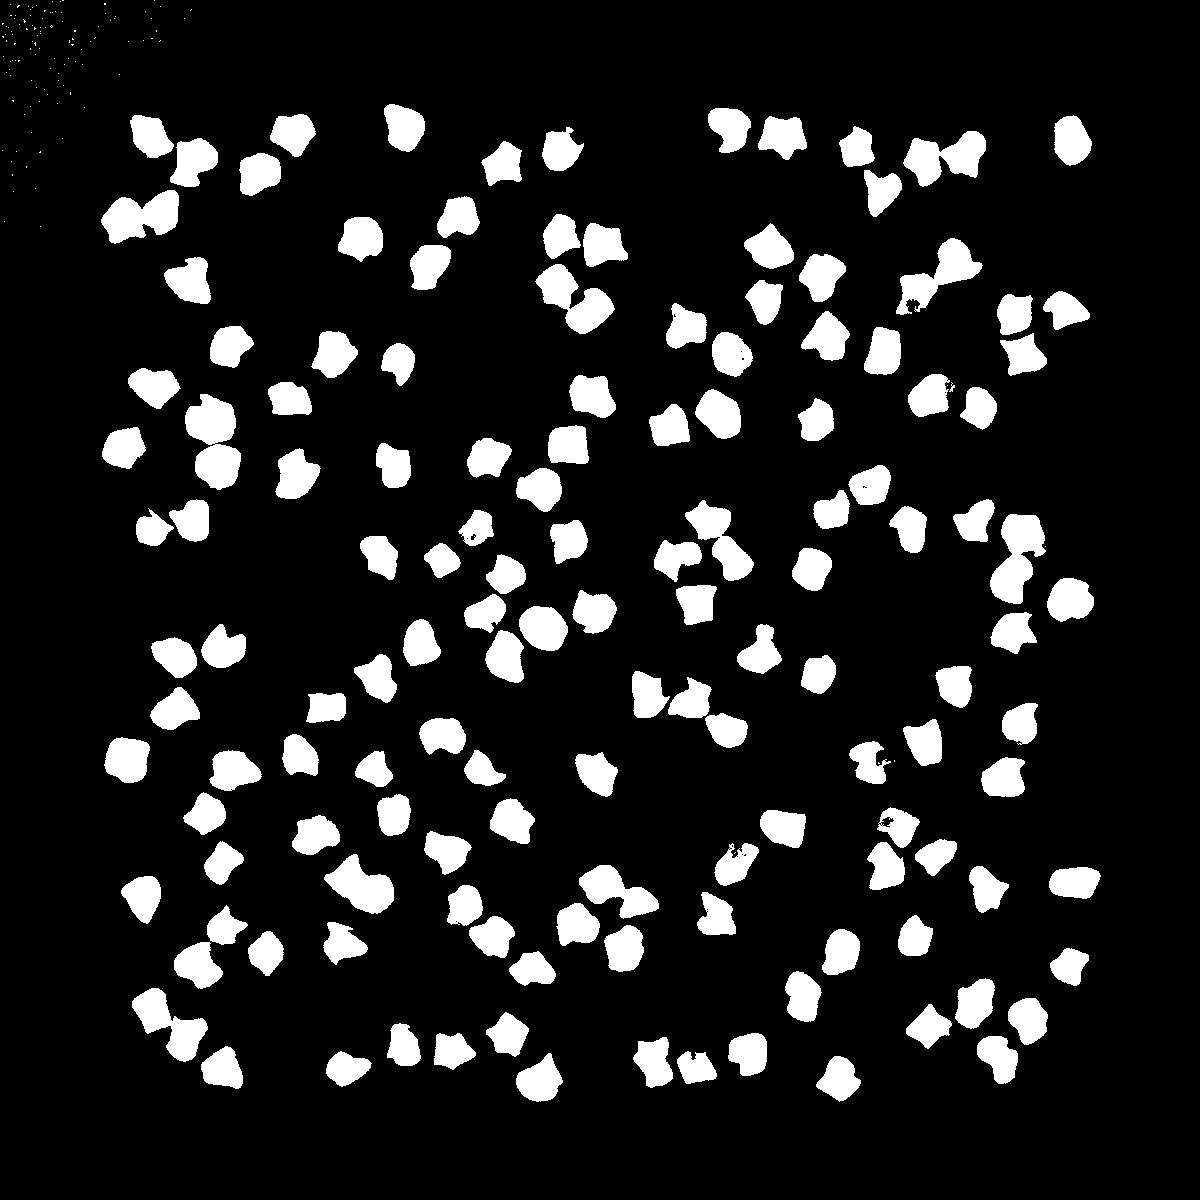
\includegraphics[width=\textwidth]{segmentation_thresholding_74_illuminated.png}
        \caption{Segmentation 6}
        \label{Segmentation6}
    \end{subfigure}

    \caption{Different segmentations of cells image}
    \label{fig:segmentation_results}
\end{figure}



Figure \ref{fig:segmentation_results} shows the evaluation of different segmented images, produced from methods of illumination correction and basic thresholding techniques as mentioned in Section \ref{sec: thresholding_and_illumination_correction}. Below are their results presented in the table:

\begin{table}[H]
    \centering
    \begin{tabular}{l|c|c|c}
         \textbf{Segmentation Figure} & \textbf{Threshold} & \textbf{Sensitvity} & \textbf{Specificity} \\
    \hline
        \ref{Segmentation1} & 92 & 0.70 & 0.99 \\ \hline
        \ref{Segmentation2} & 105 & 0.40 & 0.99 \\ \hline
        \ref{Segmentation3} & 60 & 0.99 & 0.72 \\ \hline
        \ref{Segmentation4} & 88 & 0.78 & 0.99 \\ \hline
        \ref{Segmentation5} & 84 & 0.86 & 0.99 \\ \hline
        \ref{Segmentation6} & 74 & 0.97 & 0.99 \\ \hline
    \end{tabular}
    \caption{Sensitivity and Specificity Results}
    \label{tab:sensitivity_and_Specificity_results}
\end{table}

By comparing the segmented images in Figure \ref{fig:segmentation_results} with the referenced cell image in Figure \ref{fig:cells_referenced}, we assessed Sensitivity and Specificity of these different segmentations. The outcomes of this evaluation are summarized in Table \ref{tab:sensitivity_and_Specificity_results}. Figure \ref{Segmentation6} provides the best balance between sensitivity (0.97) and specificity (0.99), making it the most effective overall for this dataset. 

In addition to Sensitivity and Specificity, \textbf{the Dice Coefficient} and the \textbf{Jaccard Index} are also crucial measures for evaluating the quality of image segmentation. The Dice Coefficient, also known as the F1 Score, is useful in assessing overlap as it considers both precision and recall to measure the similarity between the segmented output and the ground truth. Alternatively, the Jaccard Index, also referred to as Intersection over Union, evaluates accuracy by calculating the proportion of the intersection to the union of expected and observed segments. These metrics have also been utilized to assess Skin Lesion \cite{setiawan_skin_lesion_metrics}.

\subsection{Otsu's Method}

Otsu's method is a popular thresholding technique in image processing, commonly used for image segmentation. Developed by Nobuyuki Otsu in 1979. This technique automatically determines the optimal threshold for separating an image's pixels into foreground and background. This is accomplished by reducing differences within the same class and increasing differences between the two pixel classes. Otsu's method calculates the threshold value by assessing the histogram of the image, which shows the spread of pixel intensities. Pixels below the threshold are considered background, while those exceeding it are labeled as foreground \cite{otsu}.

The \textbf{main objective of Otsu's method} is to convert  grayscale images into binary images by analyzing the histogram of pixel intensity to find the optimal threshold for separating the image into two groups. The method identifies every possible threshold and selects the one that maximizes the variance between classes, enabling the effective differentiation between foreground and background. Due to its worldwide scope and emphasis on differences rather than specific local features such as pixel intensity lows or peaks, this technique is particularly effective in settings with changing lighting and noise levels.

Firstly, we have a normalized histogram \( h\), where \( h(i) \) denotes the likelihood of every pixel intensity \( i \) in the image. The technique utilizes the histogram to determine the ideal threshold by maximizing the inter-class variance. Listed below are the initial equations to start with:

\begin{equation}
P_1(\theta) = \sum_{i=0}^{\theta} h(i)
\label{eq:p1_equation}
\end{equation}

\begin{equation}
P_2(\theta) = 1 - P_1(\theta) = \sum_{i=\theta+1}^{L-1} h(i)
\label{eq:p2_equation}
\end{equation}

Equation \ref{eq:p1_equation} and \ref{eq:p2_equation}  represent the probabilities \( P_1(\theta) \) and \( P_2(\theta) \) that shows the likelihood of a pixel intensity falling into the background or foreground class, respectively.\( P_1(\theta) \) is the cumulative sum of the histogram values \( h(i) \) from 0 to \( \theta \), representing the number of pixels below the threshold (background). \( P_2(\theta) \) is the sum of the histogram values from \( \theta+1 \) to \( L-1 \), representing the number of pixels above the threshold (foreground), where \( L\) is the length of all pixel intensities shown in the histogram .

Then the mean intensities for both classes are calculated. The mean intensity values \( \mu_1(\theta) \) and \( \mu_2(\theta) \) are the mean intensities of the background and foreground classes, respectively. They are calculated as:

\begin{equation}
\mu_1(\theta) = \frac{1}{P_1(\theta)} \cdot \sum_{i=0}^{\theta} (i + 1) h(i)
\end{equation}

\begin{equation}
\mu_2(\theta) = \frac{1}{P_2(\theta)} \cdot \sum_{i=\theta+1}^{L-1} (i + 1) h(i)
\end{equation}

where \( \mu_1(\theta) \) is the weighted sum of the intensity levels up to the threshold \( \theta \), divided by the probability \( P_1(\theta) \), giving the mean intensity of the background. Similarly, \( \mu_2(\theta) \) is the weighted sum of the intensity levels from \( \theta+1 \) to \( L-1 \), divided by the probability \( P_2(\theta) \), giving the mean intensity of the foreground.

The inter-class variance \( \sigma_B^2(\theta) \) is a measure of how distinct the two classes (foreground and background) are. It is calculated as:

\begin{equation}
\sigma_B^2(\theta) = P_1(\theta) \cdot P_2(\theta) \cdot \left(\mu_1(\theta) - \mu_2(\theta)\right)^2
\label{eq:sigma_squared_equation}
\end{equation}

Here, Equation \ref{eq:sigma_squared_equation} shows the formula for calculating \( \sigma_B^2(\theta) \) representing the inter variance for a given threshold \( \theta \). The larger this variance, the better the separation between the two classes. \( P_1(\theta) \) and \( P_2(\theta) \) are the probabilities of the classes, and \( \mu_1(\theta) \) and \( \mu_2(\theta) \) are their respective mean intensities. The point where we get the maximum variance between the two classes defines our optimal threshold.

Although Otsu's method is frequently utilized, \textbf{it has some limitations}. Initially, it assumes that the image histogram displays bimodality, showing two distinct peaks that symbolize the foreground and background. However, the technique may not be effective if the histogram has a single peak or multiple peaks \cite{sezgin_image_techniques}. The limitation is discussed in the referenced paper, as the authors aimed to evaluate how different image segmentation techniques perform on a variety of image categories. They found out that Otsu's technique is limited because it needs a bimodal histogram, which reduces its effectiveness on images with unimodal or multimodal distributions. Moreover, noise and non-uniform illumination can affect Otsu's method, changing the histogram and leading to poor threshold selection, possibly compromising segmentation accuracy \cite{huang_minimizing_fuzziness}. The authors of this paper explore various methods for image thresholding in a specific example, assessing their performance under conditions of noise and uneven lighting. They specifically assess Otsu's method, noting that while it is effective in certain scenarios, its reliance on general histogram characteristics makes it vulnerable to noise and uneven lighting disruptions.

For the purpose of this report, Otsu's method was applied to segment the given image as shown in Figure \ref{fig:figurecell} by determining the optimal threshold value, which was found to be \textbf{92}. This threshold effectively separates the image into two distinct classes: foreground and background. Specifically, pixels with intensities below 92 were classified as background, while those above this threshold were classified as foreground. The segmentation result demonstrates the method's ability to distinguish between different regions of the image based on pixel intensity distribution.

To illustrate this using Otsu's method, the following figure presents the resulted segmented image

\begin{figure}[h]
    \centering
    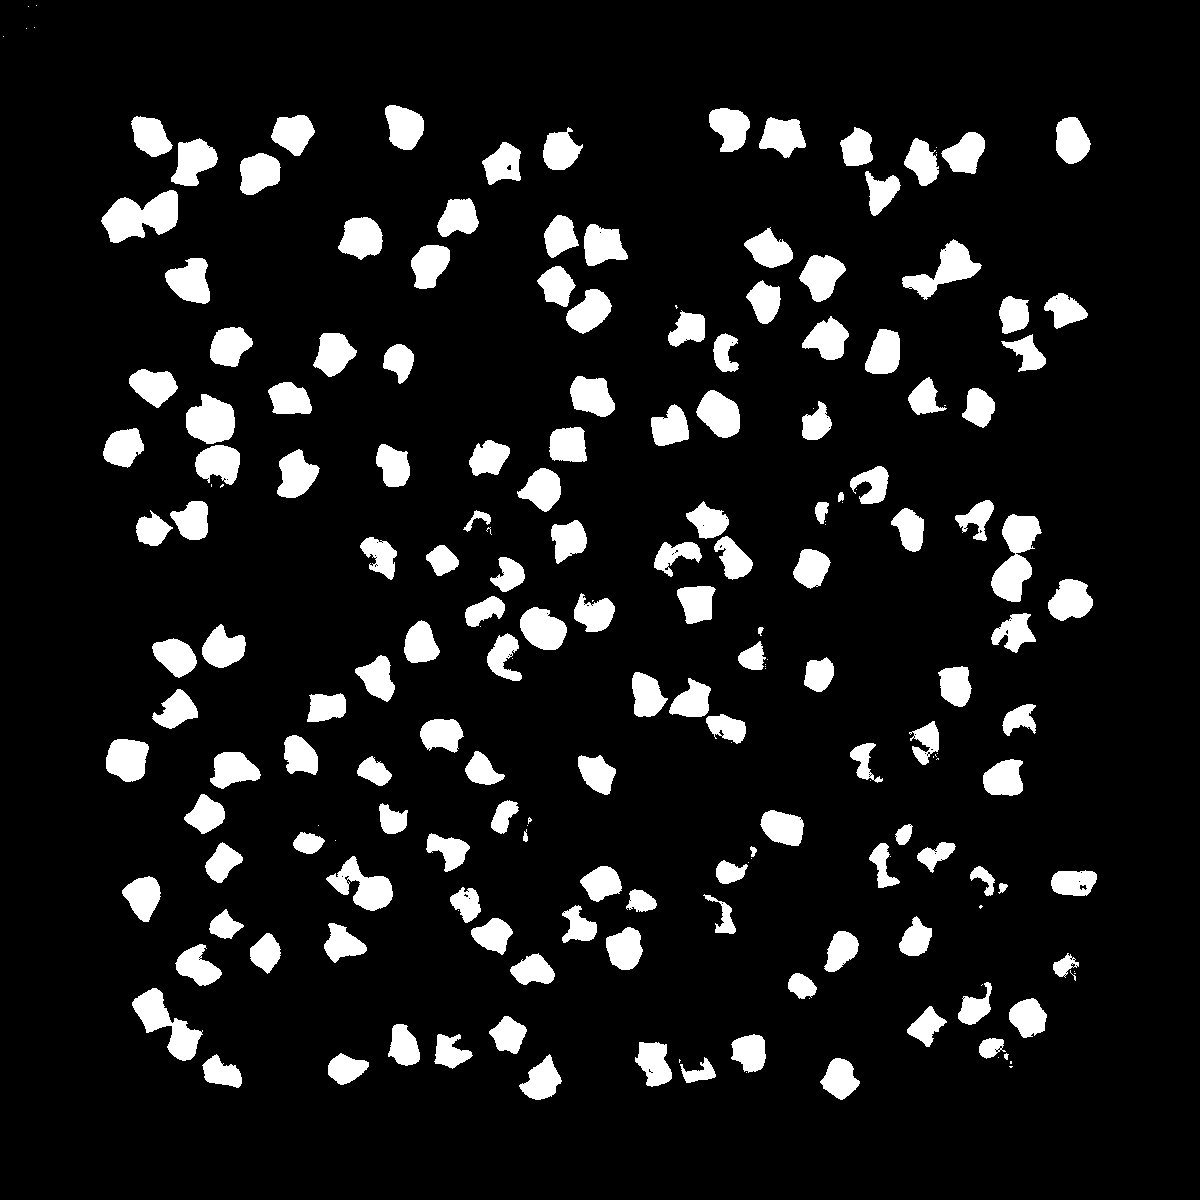
\includegraphics[width=0.3\linewidth]{otsu_segmentation.jpg}
    \caption{Otsu Segmented Image with optimal threshold t = 92}
    \label{fig:otsu_segmentation}
\end{figure}

Figure \ref{fig:otsu_segmentation} shows that after applying Otsu's method on the original image of cells, shown in Figure \ref{fig:figurecell}, we got the following result which was able to classify foreground and background pixels based on maximum intra class variance value, which was found at a \textbf{threshold value of 92}.

When addressing the problem of selecting an optimal threshold in otsu method, it is important to understand that why this threshold is selected on the integration rather than differentiation of the histogram as Otsu also mentions this in his original publication "An optimal threshold is selected automatically and stably, not based on the differentiation (i.e. a local property such as valley), but on the integration (i.e., a global property) of the histogram.", cited in \cite{otsu}. The term \textbf{"integration"} here implies that the method considers the overall distribution of pixel intensities across the entire image, rather than focusing on specific points or small regions. By integrating the information across the entire histogram, Otsu's method is able to determine a threshold that maximizes the separation between classes globally, which tends to produce more stable and reliable results in various conditions. 

 In comparison to the naive thresholding method as described in Section \ref{sec: thresholding_and_illumination_correction} where we set a threshold based on simple metrics like a fixed value, Otsu's method is more applicable. Although the naive method is computationally efficient, it lacked the adaptability needed for different image conditions. Unlike Otsu's method, which calculates an optimal threshold by analyzing the entire image histogram, the naive method didn't consider the pixel intensity distribution, leading to inferior results in images with varying lighting or noise. Otsu’s method, while more adaptive, requires greater computational effort. The following figures shows the difference between the naive thresholding method and the Ostu based segmented image based on Figure\ref{fig:figurecell}.

\begin{figure}[H]
    \centering
    \begin{subfigure}[b]{0.4\textwidth}
        \centering
        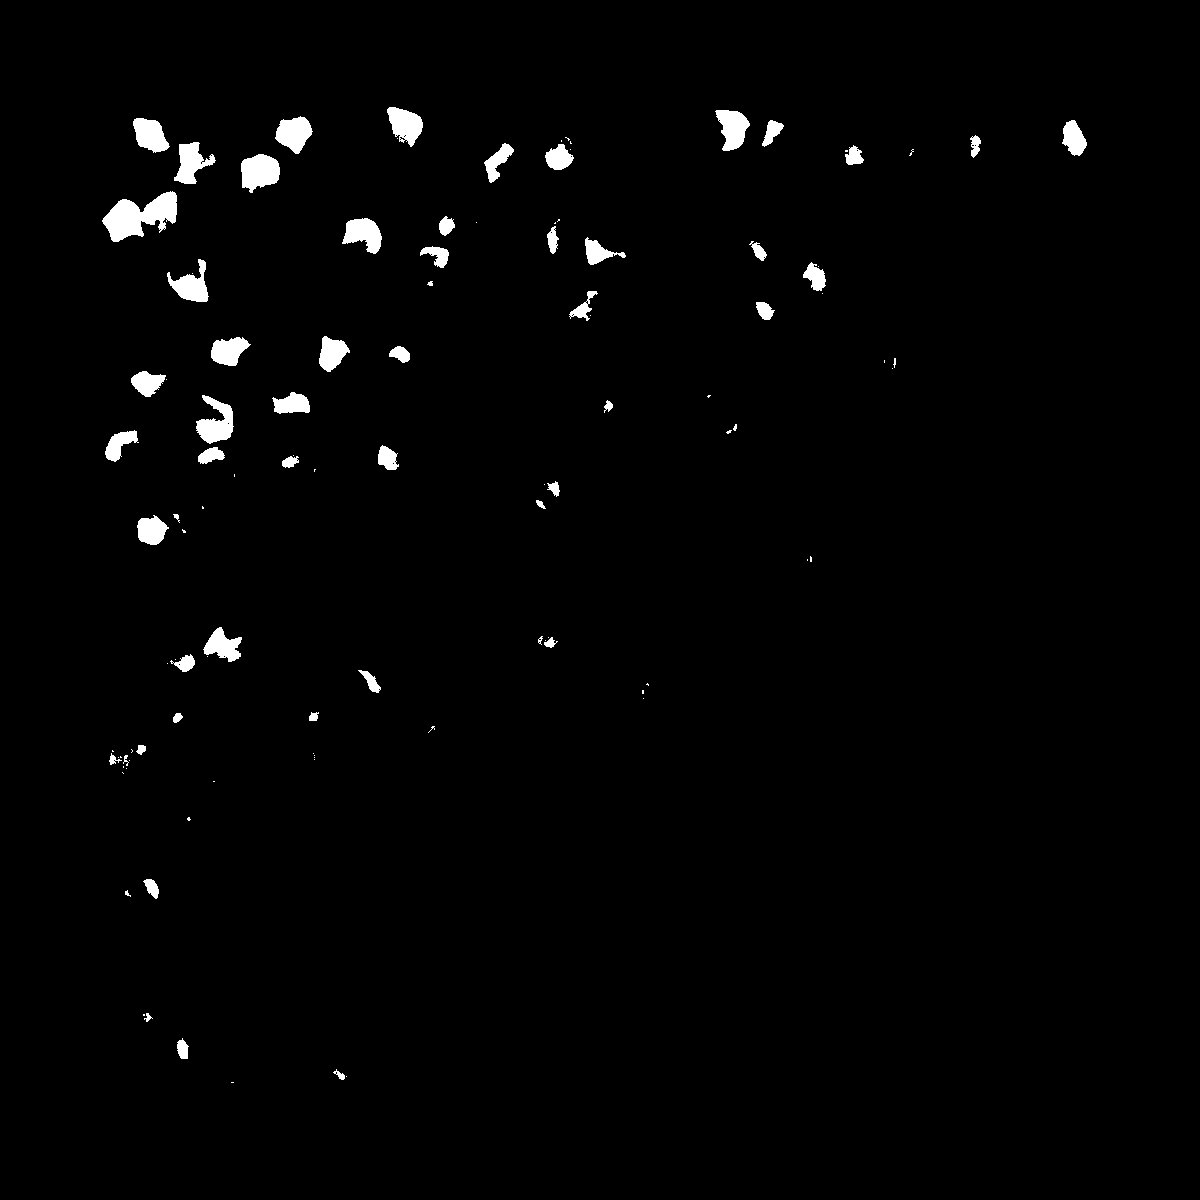
\includegraphics[width=\textwidth]{naive_thresholding_based_img.jpg}
        \caption{Naive Thresholding with t = 128}
        \label{fig:naive_thresholding_based_img}
    \end{subfigure}
    \hspace{1cm} % Adjust space between images as needed
    \begin{subfigure}[b]{0.4\textwidth}
        \centering
        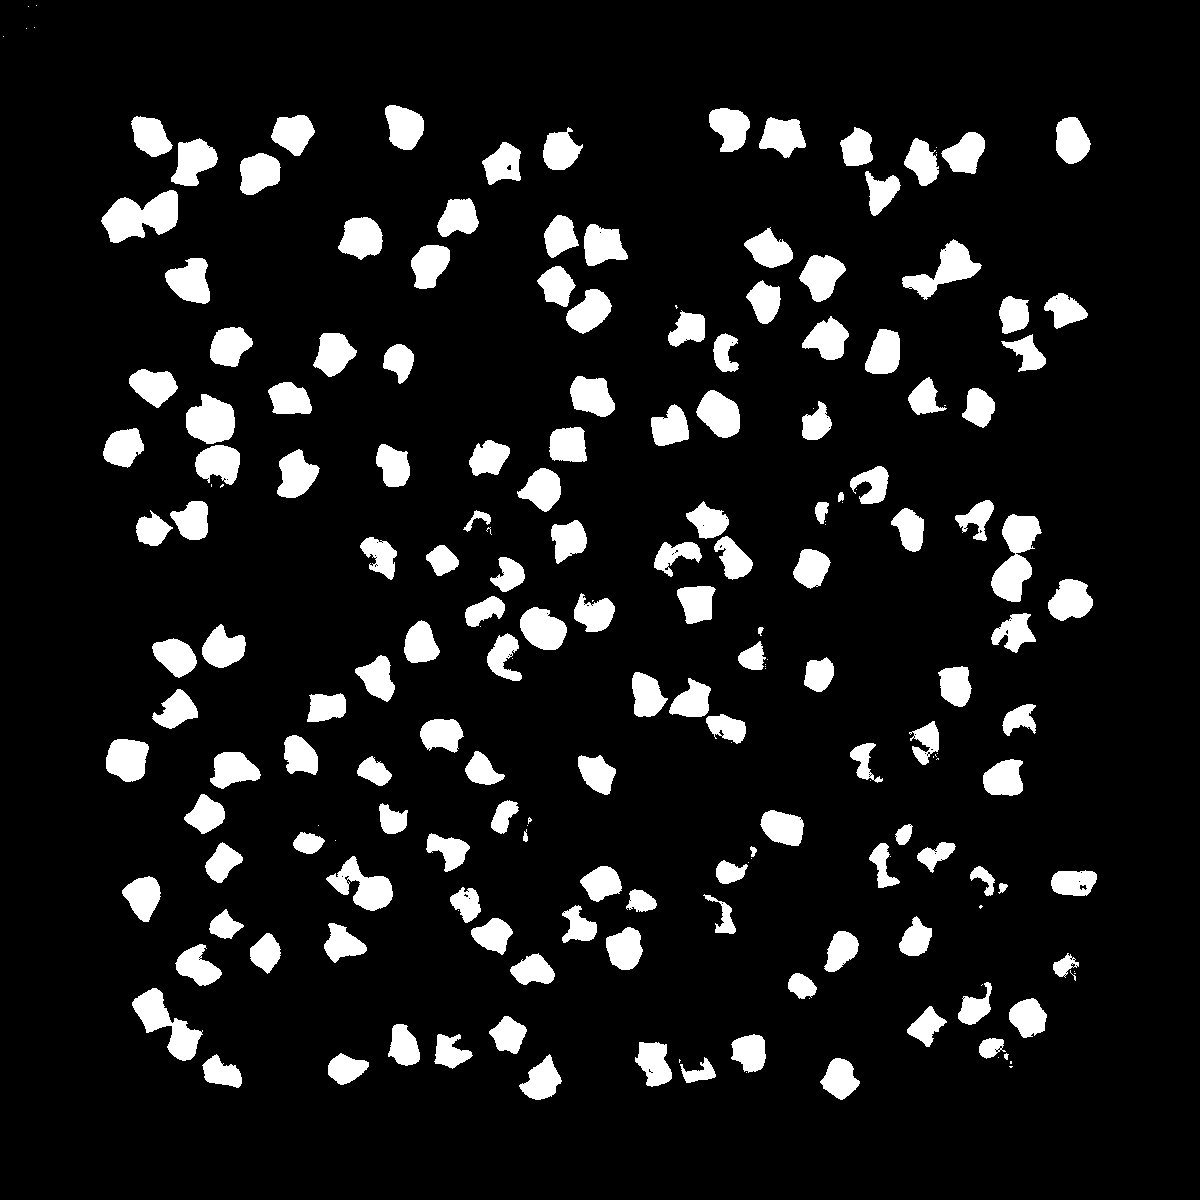
\includegraphics[width=\textwidth]{otsu_segmentation.jpg}
        \caption{Otsu Thresholding Segmentation}
        \label{fig:otsu_based_segmented_image}
    \end{subfigure}
    \caption{Comparison of Naive vs. Otsu's Thresholding on Cell Image}
    \label{fig:comparison_between_naive_and_threshold}
\end{figure}

The key difference between the above sub figures shown in \textbf{Figure \ref{fig:comparison_between_naive_and_threshold}} lies in the effectiveness of segmentation. The Naive Thresholding with t = 128 results in incomplete segmentation with many cells either not fully captured or merged into the background. In contrast, Otsu's Thresholding Segmentation produces a more accurate and complete separation of the cells from the background, demonstrating its ability to adapt to varying intensity levels within the image.
 
Despite its robustness, Otsu's method has several \textbf{shortcomings}. One major issue is its sensitivity to noise. Noise can distort the histogram, leading to incorrect thresholding. \textbf{Modern approaches} such as adaptive thresholding or local thresholding algorithms, like \textbf{Sauvola’s method}, address this limitation by computing thresholds for smaller regions of the image \cite{sauvola_adaptive_binarization}. This method improves upon traditional global thresholding techniques by calculating the threshold for each pixel based on the local mean and standard deviation within a neighborhood around that pixel, being more resilient to noise and lighting variations, particularly in scenarios like document image processing where conditions may vary significantly across the image. Additionally, Otsu's method is inherently designed for bimodal histograms, limiting it to two classes. The method might struggle to accurately segment images with more complex distributions, like multimodal ones. Modern alternatives such as k-means clustering or techniques based on machine learning can manage several classes by examining the image in greater detail and leveraging labeled data to enhance segmentation precision. A modern approach of using \textbf{Fully Convolutional Neural Networks} managed to address this issue by introducing a model that could predict labels for individual pixels, leading to improved segmentation in complex images \cite{long_fcn_segmentation}. These networks were trained to categorize each pixel into various classes, enabling thorough segmentation in complex images. FCNs are very powerful as they can be trained on extensive datasets and adapt effectively to different segmentation tasks, making them well-suited for intricate, multimodal images.

\subsection{Edge-detection}
\label{sec:edgedetection}
Edge detection, an essential stage in image processing, is utilized to recognize the borders of objects in an image. Typically, these boundaries align with regions containing a noticeable change in pixel brightness. Precise edge detection is essential for numerous tasks like computer vision, image segmentation, and object recognition. We applied the Sobel, Scharr, and Prewitt edge detection filters to Figure\ref{fig:figurecell} for this task. All of the edge detection filters utilized for this task rely on gradient operators that assess the rate of change in pixel brightness throughout an image. By applying filters to the original image, edges can be detected in either horizontal (X) or vertical (Y) orientations through the calculation of gradients in both directions.

The \textbf{Sobel filter} is among the edge detection operators that are frequently utilized. Two 3x3 convolution filters, one detecting horizontal edges (SobelX) and the other vertical edges (SobelY), are applied to calculate the image intensity gradient. The kernels' design emphasizes the regions with high spatial frequency that are associated with edges. This filter operator utilizes dual 3x3 convolution kernels for approximating the gradients in the horizontal (\(X\)) and vertical (\(Y\)) orientations, as shown below:

\begin{equation}
X = 
\begin{bmatrix}
1 & 0 & -1 \\
2 & 0 & -2 \\
1 & 0 & -1
\end{bmatrix},
\quad
Y = 
\begin{bmatrix}
1 & 2 & 1 \\
0 & 0 & 0 \\
-1 & -2 & -1
\end{bmatrix}.
\end{equation}

where by applying these two kernels in X and Y direction, on an Image (\(I\)), as shown in Figure \ref{fig:figurecell}, results in two derivatives, named as \(G_x\) and \(G_y\). The image gradient is then calculated using euclidean norm over both derivatives at each pixel in the image:

\begin{equation}
G = \sqrt{G_x^2 + G_y^2}.
\label{eq:img_gradient}
\end{equation}   

The \textbf{Scharr filter} is a more accurate version of the Sobel filter, designed to enhance gradient magnitude precision and rotational symmetry. This filter is particularly useful when precise edge recognition is needed, such as in photos with complex details or subtle changes in intensity, especially in the detection of diagnol edges . Below are the two 3x3 convolution filters used to calculate the gradients in the horizontal (\(X\)) and vertical (\(Y\)) directions for this filter.

\begin{equation}
X = 
\begin{bmatrix}
47 & 0 & -47 \\
162 & 0 & -162 \\
47 & 0 & -47
\end{bmatrix},
\quad
Y = 
\begin{bmatrix}
47 & 162 & 47 \\
0 & 0 & 0 \\
-47 & -162 & -47
\end{bmatrix}.
\end{equation}

The gradient is calculated in the same manner as Sobel, shown in Equation \ref{eq:img_gradient}. This  filter is known for its higher precision in detecting edges. This is because its kernels are optimized to better approximate the derivative of the image.

Another gradient-based edge detector is the \textbf{Prewitt filter}. It also uses two 3x3 convolution kernels to calculate the gradient of the image intensity, just like the Sobel filter, but with a slightly simpler set of convolution kernels. The Prewitt operator is generally less sensitive to noise than Sobel, but it also provides a less precise gradient approximation. The kernels used for this filter are:

\begin{equation}
X = 
\begin{bmatrix}
1 & 0 & -1 \\
1 & 0 & -1 \\
1 & 0 & -1
\end{bmatrix},
\quad
Y = 
\begin{bmatrix}
1 & 1 & 1 \\
0 & 0 & 0 \\
-1 & -1 & -1
\end{bmatrix}.
\end{equation}

and the gradient is again calculated in the same manner as Sobel and Scharr, given in Equation \ref{eq:img_gradient}. Prewitt filters are appropriate for situations where noise reduction is a priority since they are frequently less susceptible to noise than Sobel filters. It does, however, give a less precise approximation of the gradient.


While the Scharr, Prewitt, and Sobel filters are frequently utilized for edge detection, there are certain \textbf{limitations} that require the consideration of more sophisticated techniques. One of the primary drawbacks is their vulnerability to noise. These filters are prone to identifying fake edges because they compute the gradient of the image intensity, which is typically caused by small intensity fluctuations brought about by noise in the image \cite{gonzalez_digital_image_processing}. In real-world photos, where noise is inevitable, this problem is especially troublesome . Additionally, these filters are not as effective at detecting diagonal or curved edges since they are designed to primarily detect edges aligned with the horizontal and vertical axes. In images with complicated geometries, this directional bias may result in partial edge detection \cite{jain_machine_vision}. Furthermore, the fixed size of the convolution kernels restricts their ability to detect edges of various sizes in an image, potentially causing the loss of important details or the failure to capture bigger structures \cite{marr_edge_detection_theory}. Finally, the approximate gradient calculated by these filters often leads to inaccurate edge detection, particularly in areas with sharp gradient \cite{canny_computational_approach}. These limitations emphasize the need for more sophisticated edge detection strategies, such the Canny edge detector \cite{canny_computational_approach}, which combines approaches including edge thinning, gradient magnitude thresholding, and noise reduction to produce more precise and dependable edge detection. 

The following figures were generated to show the results of Edge detection after applying the above mentioned filters on Figure \ref{fig:figurecell}. The outermost rows and columns were ignored for simplicity. 

\begin{figure}[H]
    \centering
    \begin{subfigure}[b]{0.4\textwidth}
        \centering
        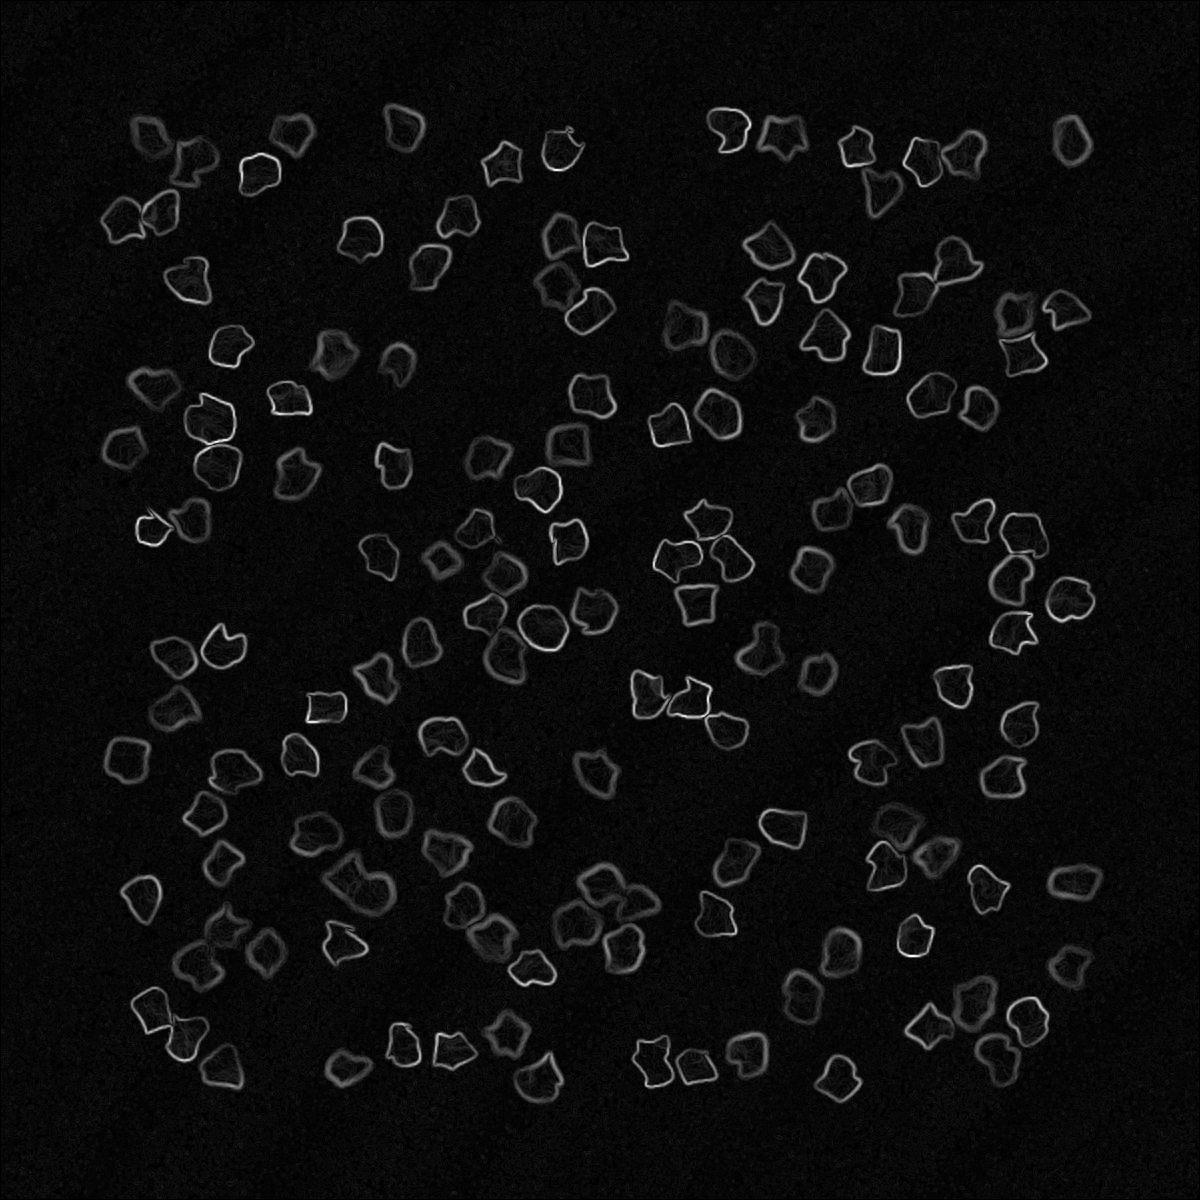
\includegraphics[width=\textwidth]{sobel_filter.png}
        \caption{Sobel Filter}
        \label{fig:sobel_img}
    \end{subfigure}
    \hspace{1cm} % Adjust space between images as needed
    \begin{subfigure}[b]{0.4\textwidth}
        \centering
        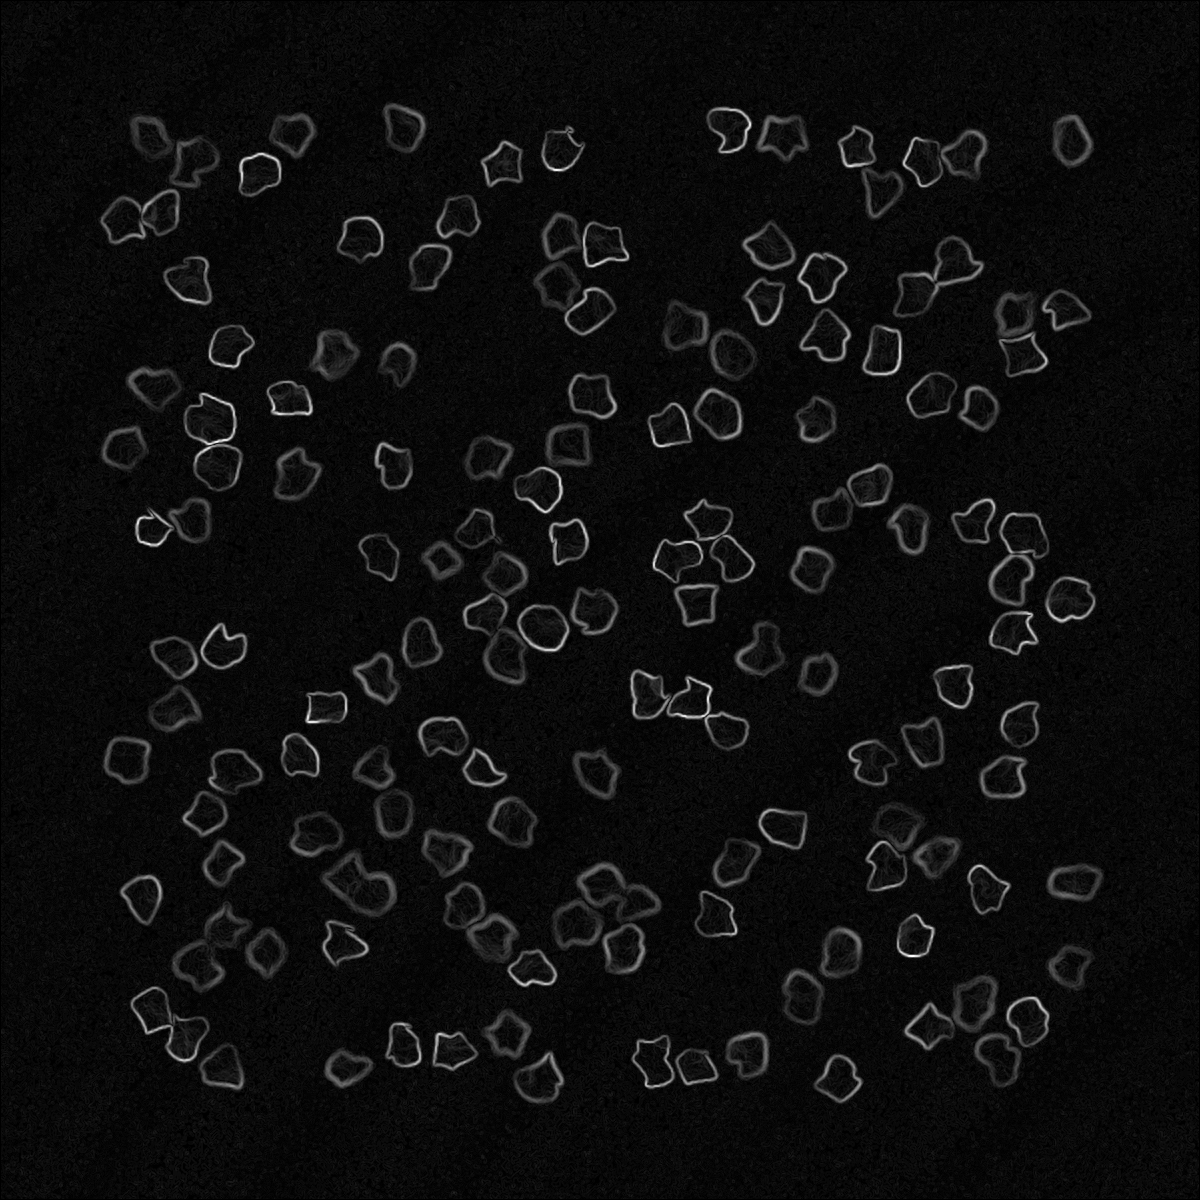
\includegraphics[width=\textwidth]{scharr_filter.png}
        \caption{Scharr Filter}
        \label{fig:scharr_filter_img}
    \end{subfigure}
        \hspace{1cm} % Adjust space between images as needed
    \begin{subfigure}[b]{0.4\textwidth}
        \centering
        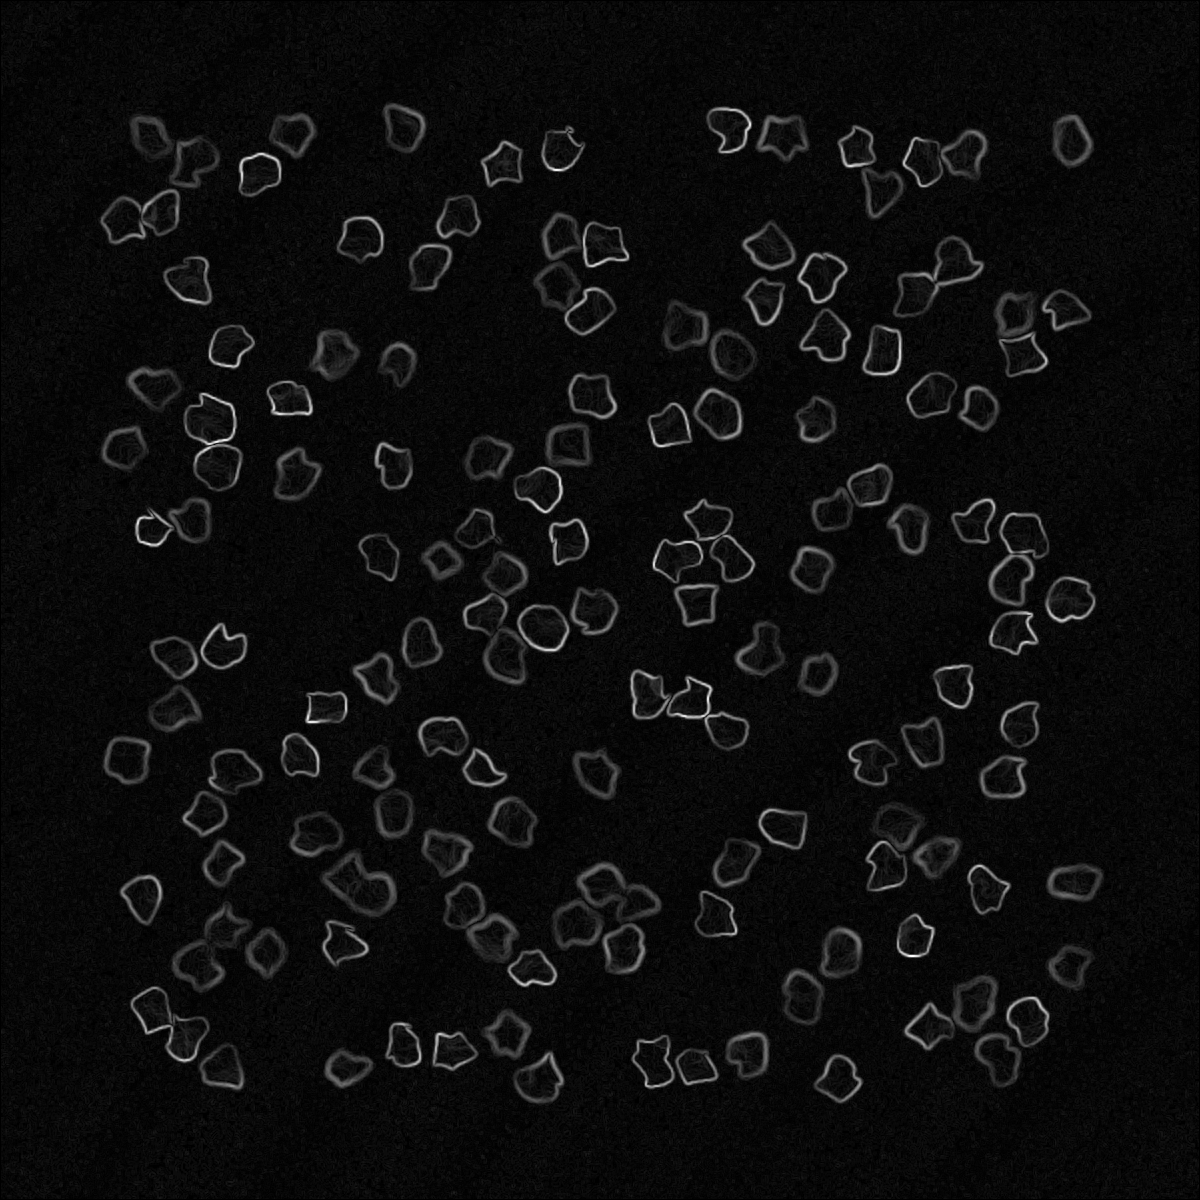
\includegraphics[width=\textwidth]{prewitt_filter.png}
        \caption{Prewitt Filter}
        \label{fig:prewitt_filter_img}
    \end{subfigure}
    \caption{Results of Primitive Edge Detection Filters}
\label{fig:comparison_between_edge_detection_filters}
\end{figure}

\textbf{In conclusion}, all three operators — Sobel, Scharr, and Prewitt effectively detect the edges of the cells particles, as shown in Figure \ref{fig:comparison_between_edge_detection_filters} given the relatively simple nature of the image. Due to the smoothness of the edges and the consistency in the image's gradient, the differences between these operators are subtle. The Scharr operator, while providing slightly sharper and more pronounced edges, aligns with its design for detecting finer edge details. However, in this specific image, these differences are not significantly pronounced.



\subsection{Canny edge detection}

A renowned method in the field of image processing, Canny Edge Detection is renowned for its ability to recognize a wide range of edges in images. John F. Canny developed the method in 1986 with the express purpose of improving edge identification by reducing noise while preserving important structural elements. It achieves this by means of a multi-phase procedure, to maximize edge detection accuracy and dependability \cite{canny_computational_approach}.


In order to accurately identify edges, the Canny Edge detection algorithm follows a sequence of important steps. In order to decrease the noise that may lead to inaccurate edge detection, an optimal Gaussian blur value is applied to the image for smoothing. Next, the method employs Sobel kernels in convolution to calculate the gradients \( G_x \) and \( G_y \) of the blurred image along the horizontal and vertical direction, respectively. Potential edges are shown by areas of fast intensity change, which are highlighted by the gradient magnitude \( |\nabla G| \). A description of these two steps can also be found in Section \ref{sec:edgedetection}. The arctangent function is utilized for determining the \textbf{direction of the gradient} like the following:

\begin{equation}
\theta(x, y) = \text{atan2}\left(G_y, G_x\right)
\end{equation}

where \(\theta(x, y)\) represents the gradient direction at each pixel, which is crucial for determining the orientation of the edges during the non-maximum suppression step.

Subsequently, Non-maximum suppression is applied to thin out the detected edges by retaining only the points that are the local maxima in the direction of the gradient, effectively reducing the edges to a single-pixel width. Subsequently, two thresholds \( T_{\text{low}} \) and \( T_{\text{high}} \) are used to categorize edges in double thresholding: edges above \( T_{\text{high}} \) are considered strong, while edges between \( T_{\text{low}} \) and \( T_{\text{high}} \) are considered weak. This concept is also known as   \textbf{Hysteresis Thresholding} which removes unneeded edges while preserving key ones by retaining weak edges only if they connect to strong edges. This method produces a more accurate edge map that accurately represents the image's outlines.

The Canny Edge Detection algorithm offers \textbf{significant advantages} over simpler methods like Sobel, Scharr, and Prewitt, particularly in handling noise, improving edge localization, and preserving edge connectivity. The primitive methods, that directly compute image gradients are very prone to noise, leading to frequent generation of incorrect edges. On the other hand, the Canny algorithm starts by applying a Gaussian blur to minimize noise and improve the precision of edge detection. Also, primitive edge detection techniques also result in thicker edges that are less accurately positioned because of basic thresholding. Canny tackles this issue by implementing non-maximum suppression, making sure that edges are both slim and accurately positioned. Additionally, Canny stands out in preserving edge connectivity, a task that simpler techniques frequently find challenging in noisy settings. By implementing double thresholding and hysteresis-based edge tracking, it retains only the crucial, connected edges, resulting in a more dependable and uninterrupted edge detection.

In general, the Canny algorithm outperforms simpler methods by efficiently decreasing noise, precisely identifying edges, and guaranteeing connectivity, making it a more reliable option for edge detection. The parameters selected, notably the Gaussian blur sigma (\(\sigma\)) and the upper and lower thresholds, have a substantial impact on the effectiveness of the Canny Edge Detection algorithm. These parameters determine the algorithm's efficiency to detecting edges and its ability to reduce noise effectively.

Three images are shown below with variations in parameter settings for thresholds and \(\sigma\) value for Gaussian blur, implemented on the same cellular structure image, as seen in Figure \ref{fig:figurecell}.

\begin{figure}[H]
    \centering
    \begin{subfigure}[b]{0.3\textwidth}
        \centering
        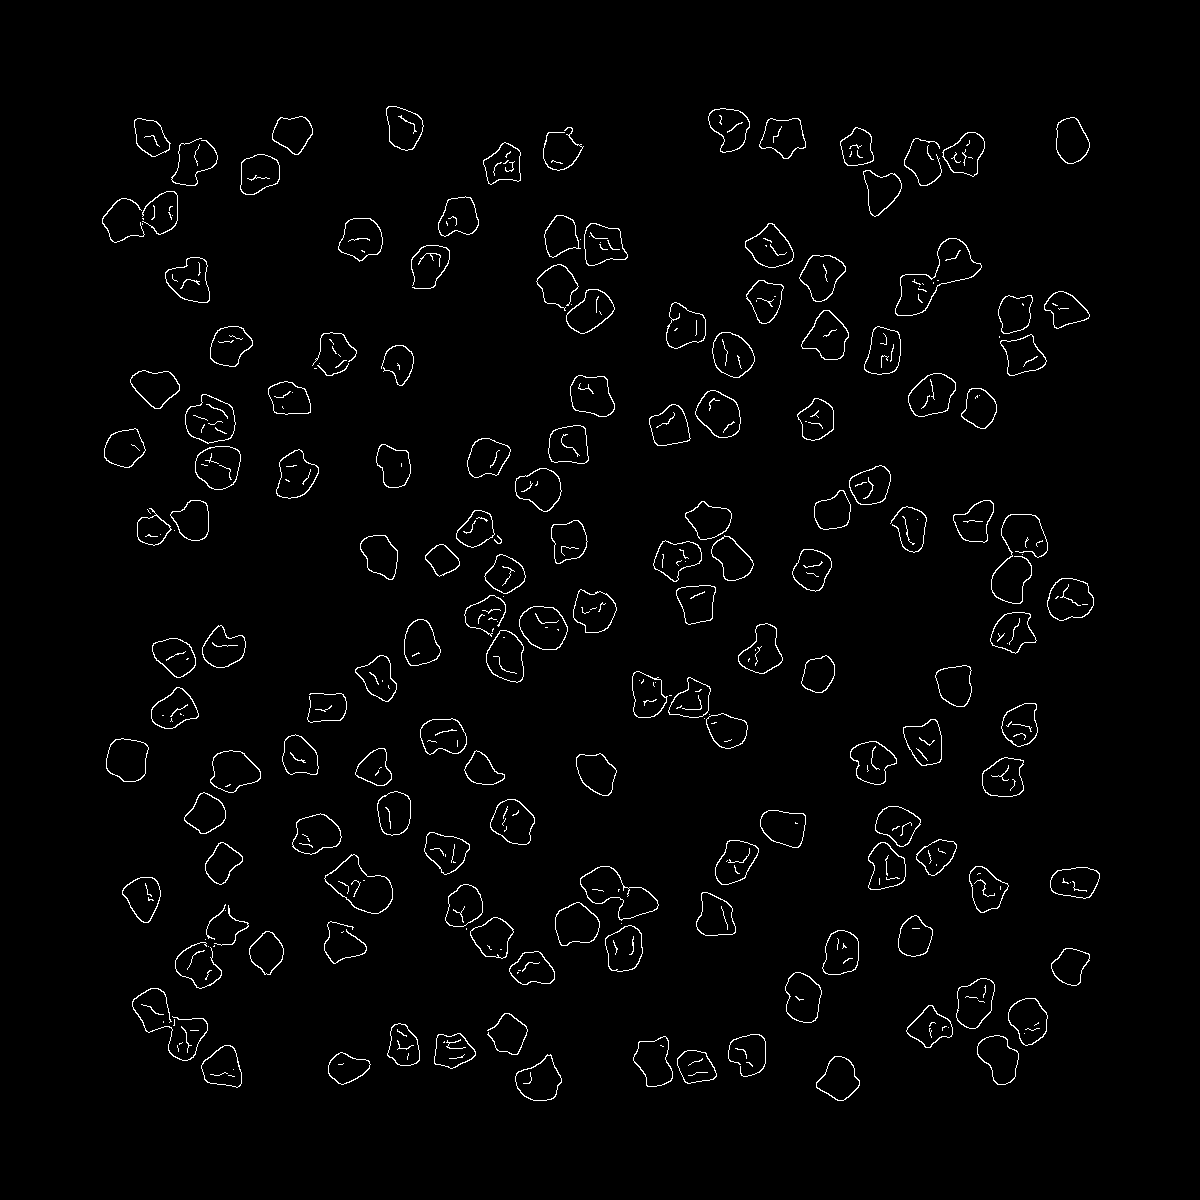
\includegraphics[width=\textwidth]{canny_edge_detection_1.png}
        \caption{First Parameter Set: \(\sigma = 2\), Thresholds = 5, 15}
        \label{fig:canny_edge_detection_img_1}
    \end{subfigure}
    \hspace{1cm} % Adjust space between images as needed
    \begin{subfigure}[b]{0.3\textwidth}
        \centering
        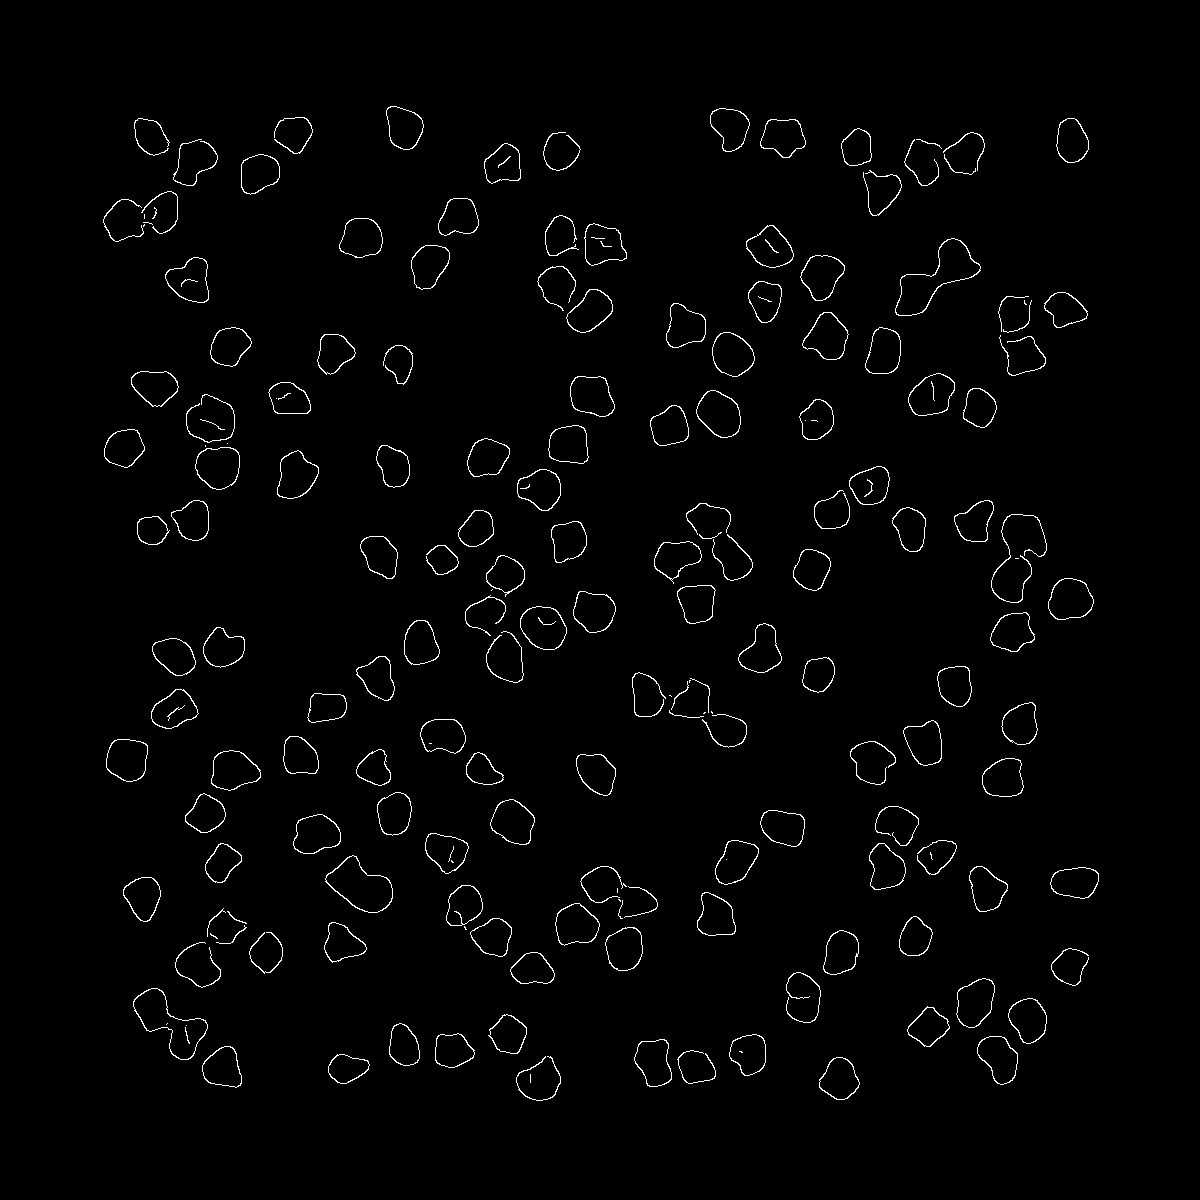
\includegraphics[width=\textwidth]{canny_edge_detection_2.png}
        \caption{Second Parameter Set: \(\sigma = 4\), Thresholds = 10, 30}
        \label{fig:canny_edge_detection_img_2}
    \end{subfigure}
     \hspace{1cm} % Adjust space between images as needed
    \begin{subfigure}[b]{0.3\textwidth}
        \centering
        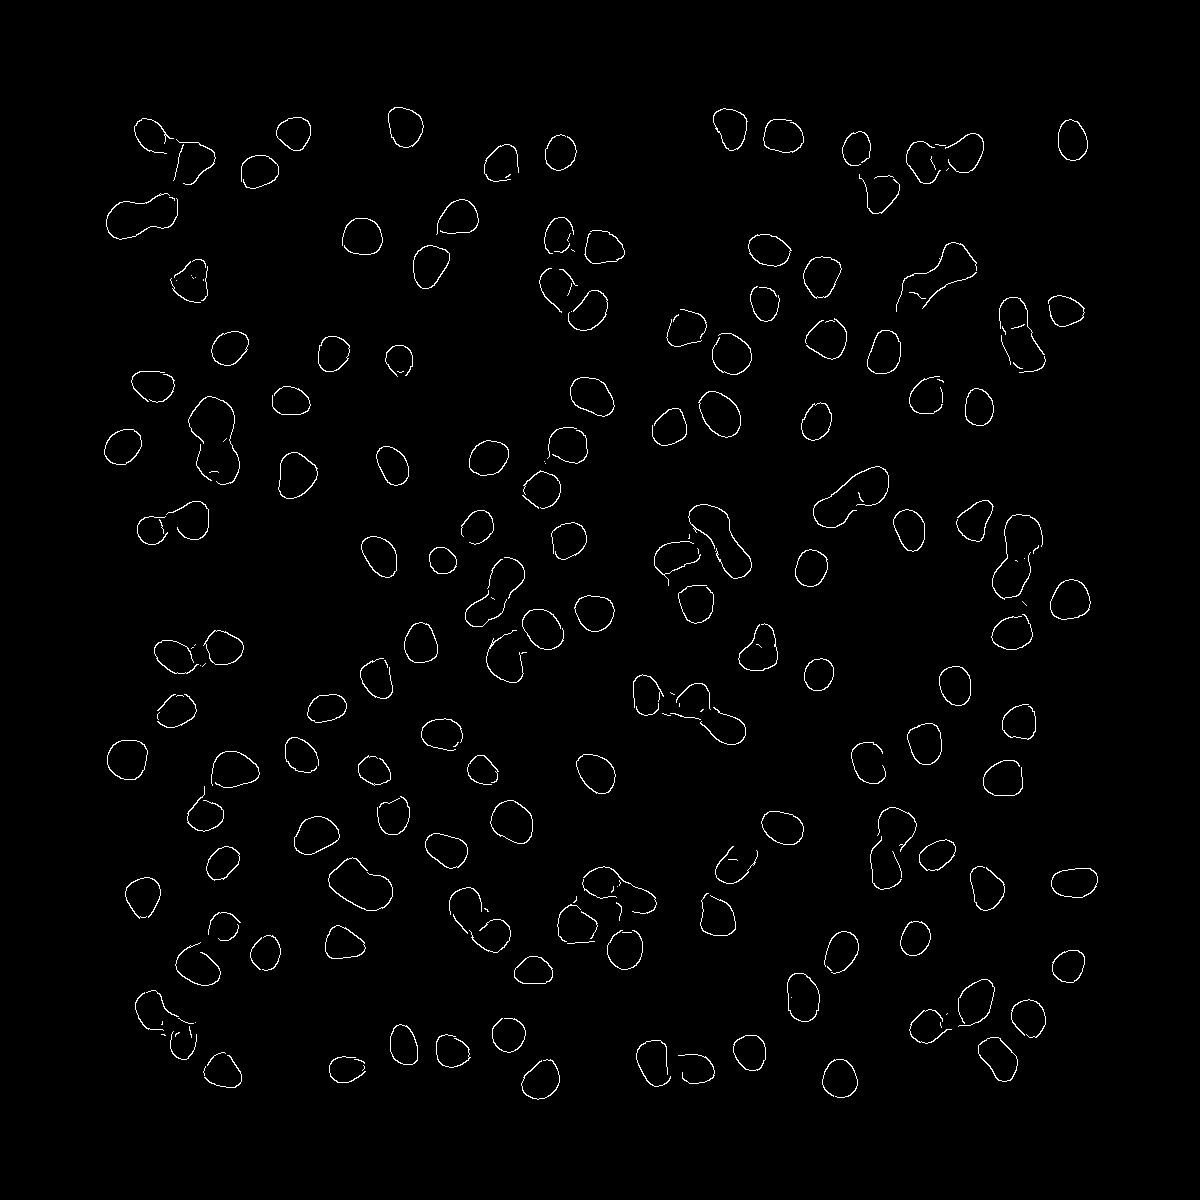
\includegraphics[width=\textwidth]{canny_edge_detection_3.png}
        \caption{Third Parameter Set: \(\sigma = 8\), Thresholds = 15, 40}
        \label{fig:canny_edge_detection_img_3}
    \end{subfigure}
    \caption{Comparison of Canny Edge Detection results with different parameter sets.}
    \label{fig:comparison_of_canny_imgs}
\end{figure}

Figure \ref{fig:canny_edge_detection_img_1} demonstrates that by applying a mild Gaussian blur, noise is decreased while detail is maintained. The thresholds enabled the identification of the majority of edges, leading to a intricate edge map. On the contrary, Figure \ref{fig:canny_edge_detection_img_2} and Figure \ref{fig:canny_edge_detection_img_3} illustrates that a higher sigma resulted in more effective smoothing, resulting in decreased noise while also causing a loss of finer details. Increasing the thresholds resulted in more discerning edge detection, only detecting the most prominent edges.

These findings demonstrate the compromises associated with selecting parameters. Decreasing sigma and thresholds leads to increased precision in detecting edges, detecting even the fainter ones. Conversely, higher values lead to smoother edges yet with less detail. The parameters selection should be based on the particular needs of the image analysis task.


% \begin{table}[]
%     \centering
%     \begin{tabular}{l|c|c|c|c|c}
%         a & b & c & d & e & f \\
%     \hline
%         1 & 2 &0.2&0.3&0.4&0.5
%     \end{tabular}
%     \caption{In case you need a table.}
%     \label{tab:my_label}
% \end{table}

\newpage
\section{Conclusion}

By creating fundamental image processing tools like Thresholding, Segmentation, and Edge detection techniques, this project has established the foundation for understanding and utilizing advanced image analysis methods. In the field of medical imaging, segmentation and edge detection are extremely important methods and should not be underestimated. These techniques play a key role in automating tasks like accurately identifying anatomical features and abnormal changes. Their use could greatly help radiologists by improving both efficiency and accuracy. Now, we will conclude this report with the current trends being used in the field of image processing. Now, we will conclude this report with the current trends being used in the field of image processing

Currently, deep learning methods, particularly \textbf{Convolutional Neural Networks} (CNN), are revolutionizing image segmentation, especially in medical applications such as organ segmentation and tumor detection. The U-Net architecture, for example, has demonstrated outstanding performance in these areas \cite{ronneberger_cnn}. Additionally, \textbf{Multi-Modal Image Fusion}, which combines data from different imaging modalities like MRI and PET, is gaining attention for its potential to enhance diagnostic precision, though it faces challenges in clinical implementation due to the complexity of data integration and computational demands \cite{james_medical_img_fusion}.

\textbf{Transfer learning} is also emerging as a solution to the challenge of limited labeled data in medical imaging. By adapting pre-trained models to specific medical tasks, it enables the rapid deployment of effective models with reduced training times, though it requires further validation across diverse clinical settings \cite{cheplygina_transfer_learning}.

Among these trends, deep learning segmentation using CNNs is the most advanced and is increasingly being incorporated into clinical practice, particularly for tumor identification and organ delineation, but still the issues for handling large amounts of training data and having enough computational power exist. In contrast, transfer learning and multi-modal image fusion remain primarily in the research stage, with their clinical application contingent on overcoming validation, regulatory, and integration challenges. Transfer learning shows potential for situations with a lack of data, but it must undergo thorough validation in various clinical settings to guarantee its dependability and applicability before widespread adoption. Likewise, the process of combining data from multiple imaging modalities in multi-modal image fusion is inhibited by the complexity and computational requirements

The report effectively showed various basic image processing techniques such as thresholding, segmentation, and edge detection, as they were successful in solving key image analysis challenges. Nevertheless, some limitations are there that could affect the overall effectiveness of these methods. One main issue is that thresholding and edge detection methods are sensitive to changes in image quality and lighting conditions. Even though histogram equalization was used to address lighting differences, the effectiveness of these techniques varied among images, leading to less than ideal results for segmentation and edge detection. Additionally, the reliance on manual parameter adjustment in techniques such as Otsu's thresholding and the Canny edge detector can lead to possible user bias and result variability. This manual intervention not just decreases reliability but also limits the scalability of these techniques when used on extensive datasets or in clinical environments. Furthermore, though these techniques are usually successful in analyzing relatively uncomplicated images, their use for more detailed medical images, which frequently contain elaborate structures, is still limited.

To address these limitations, future studies should concentrate on enhancing the dependability of these methods, particularly across various imaging settings. This could involve integrating adaptive algorithms or using machine learning methods to automatically modify parameters and enhance the management of different imaging scenarios. As research advances, these developments may transition from experimental to common clinical practice, resulting in significant improvements in diagnostic imaging and leading to more accurate and efficient medical assessments.

% Literaturverzeichnis
\newpage
\bibliographystyle{apalike}
\bibliography{Bib/literatur}

\end{document}
  